\documentclass[a4paper]{article}


\usepackage[utf8]{inputenc}    
\usepackage[T1]{fontenc}
\usepackage[francais]{babel}     
%\usepackage{hyperref}
\usepackage{graphicx}

\usepackage[colorlinks,hyperindex,bookmarks,linkcolor=blue,citecolor=blue,urlcolor=blue]{hyperref}

\usepackage{placeins}% pour \FloatBarrier (permet de placer les figures au bon endroit)


\usepackage[colorinlistoftodos]{todonotes}


\title{Edukera}
\author{Paul Dubois}
\date{12 sept. 2017}
\begin{document}
\maketitle



\tableofcontents



\section{Accéder à Edukera}



Tout d'abord, rendez-vous sur \href{https://www.edukera.com/}{le site d'Edukera} (\url{https://www.edukera.com/}).
Au moment où j'écris ces lignes, le site ressemble à cela:
\begin{figure}[h!]
\begin{center}
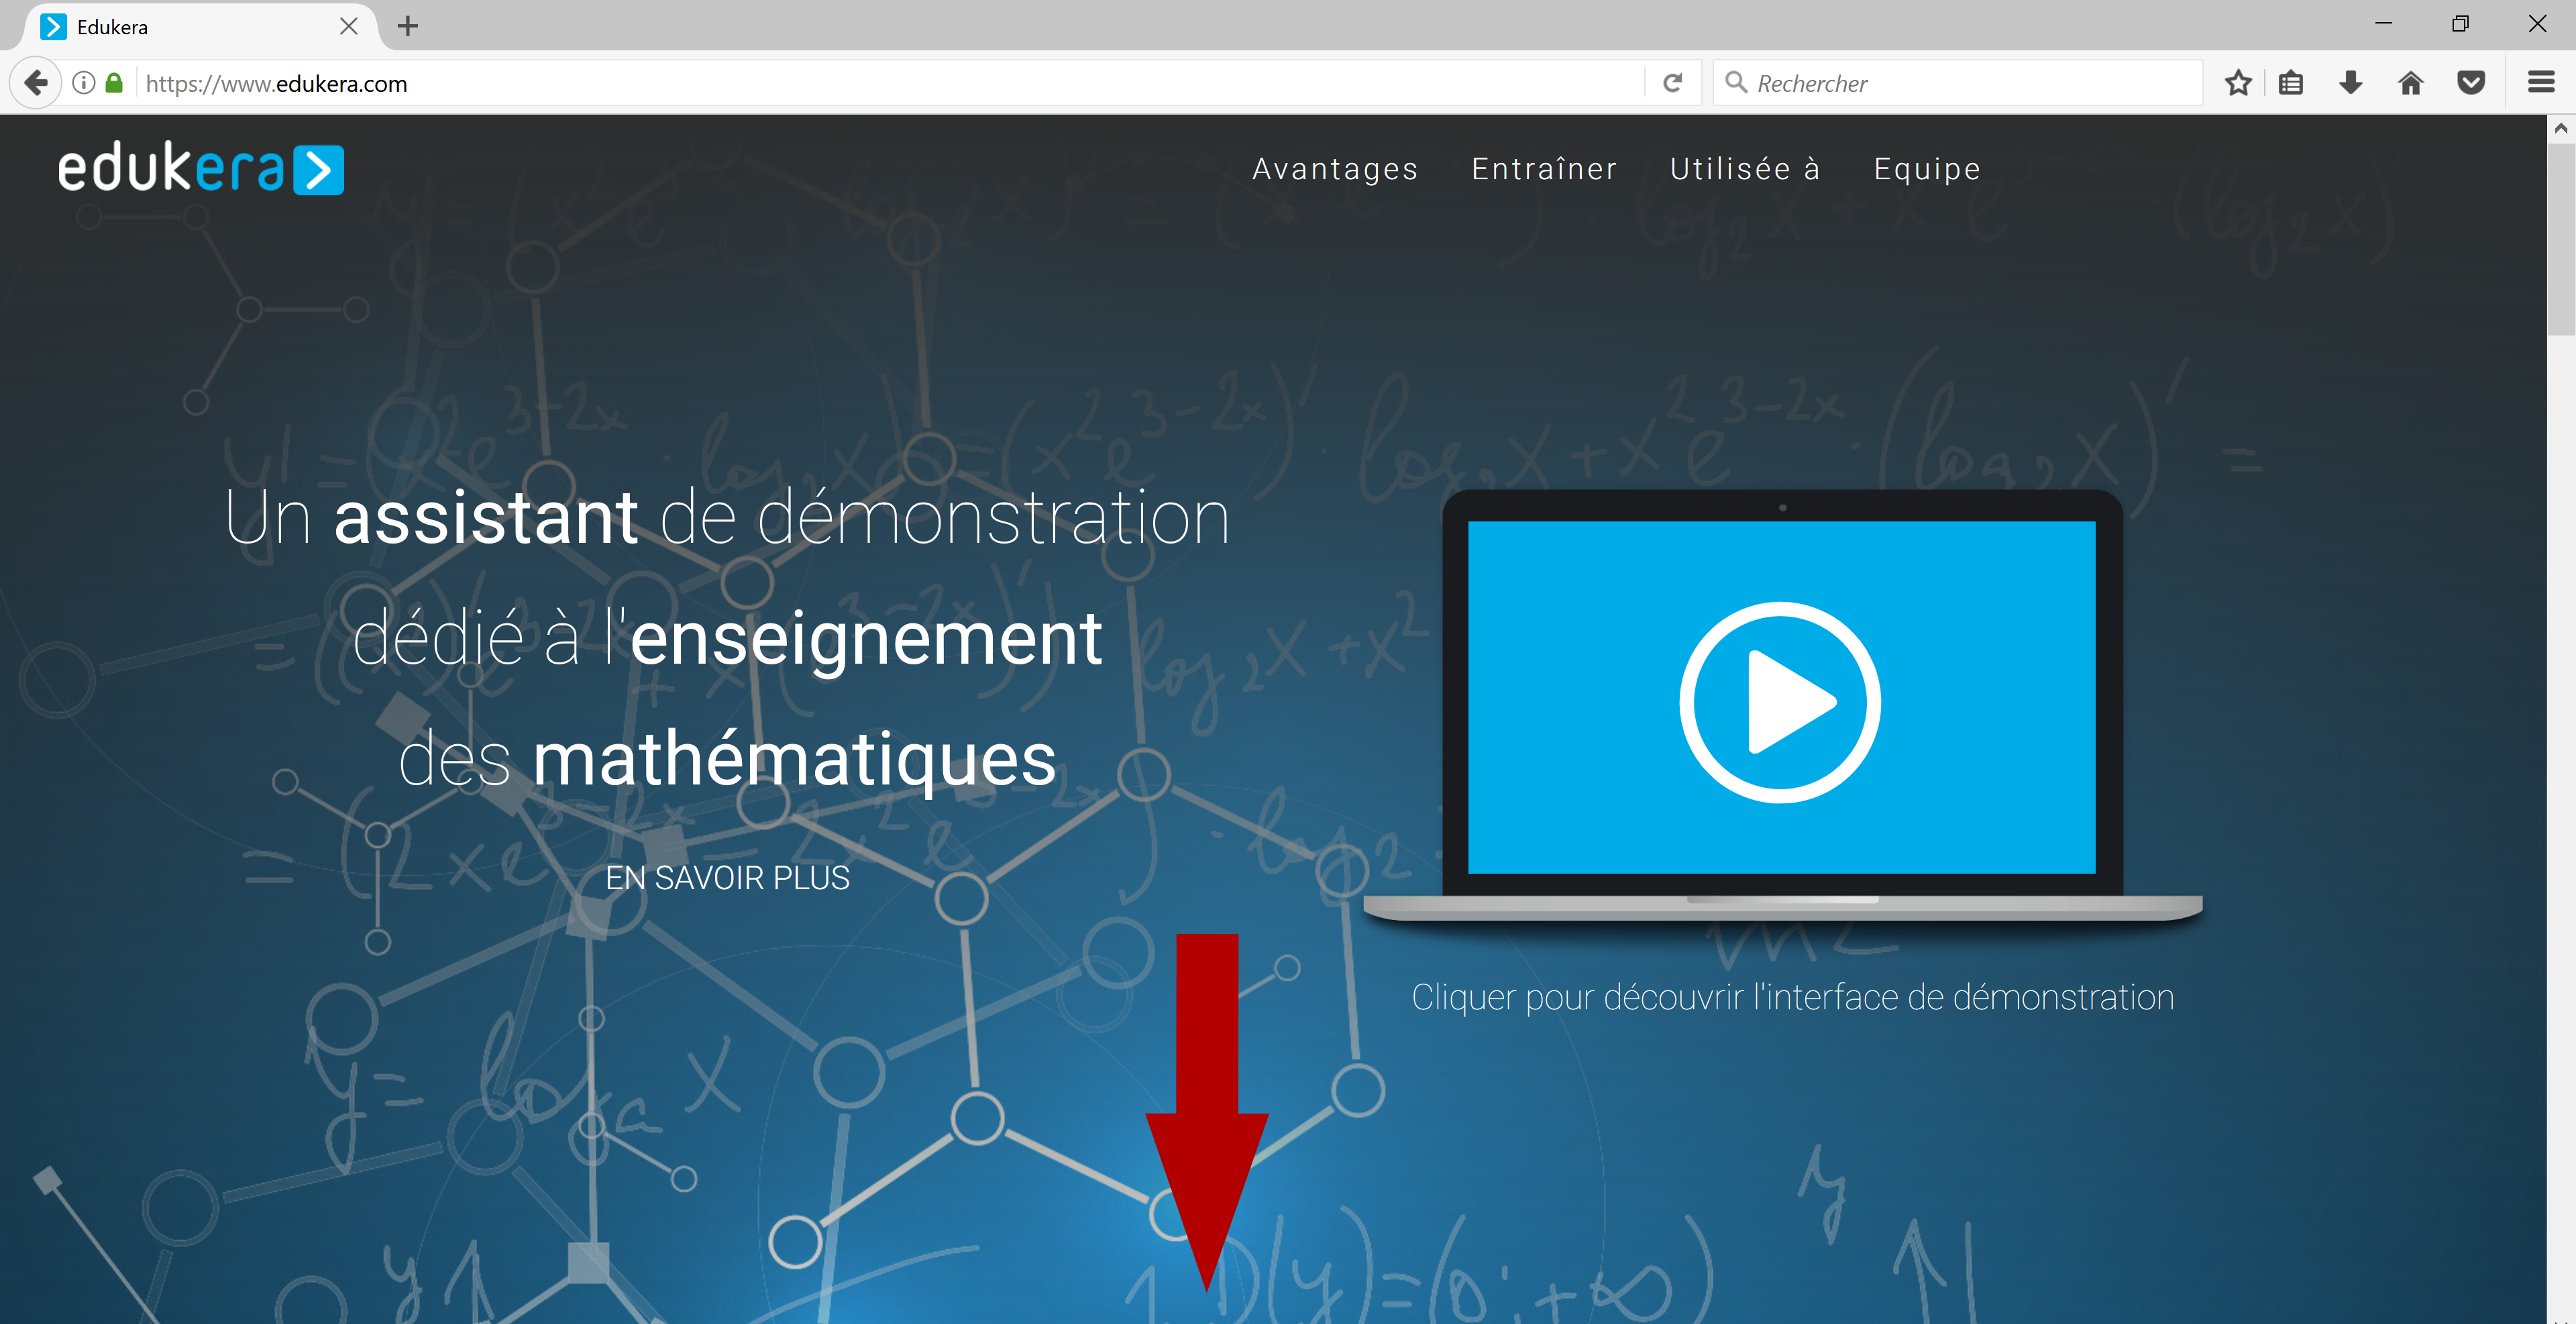
\includegraphics[scale=0.1]{img_site0.png}
\end{center}
\caption{Accueil su site Edukera}\label{im:site_edukera_haut}
\end{figure}
\FloatBarrier

Le site fait la promotion d'Edukera, mais ce qui nous intéresse est d'accéder à l'application. Si vous cliquez sur "découvrir l'interface de démonstration", vous n'accéderez pas à l'application Edukera, mais à un tutoriel. Pour accéder à Edukera, faites défiler le site vers le bas, jusqu'à ce que le bouton "Accéder à l'application" apparaisse dans le bandeau supérieur, comme dans l'image suivante:
\begin{figure}[h!]
\begin{center}
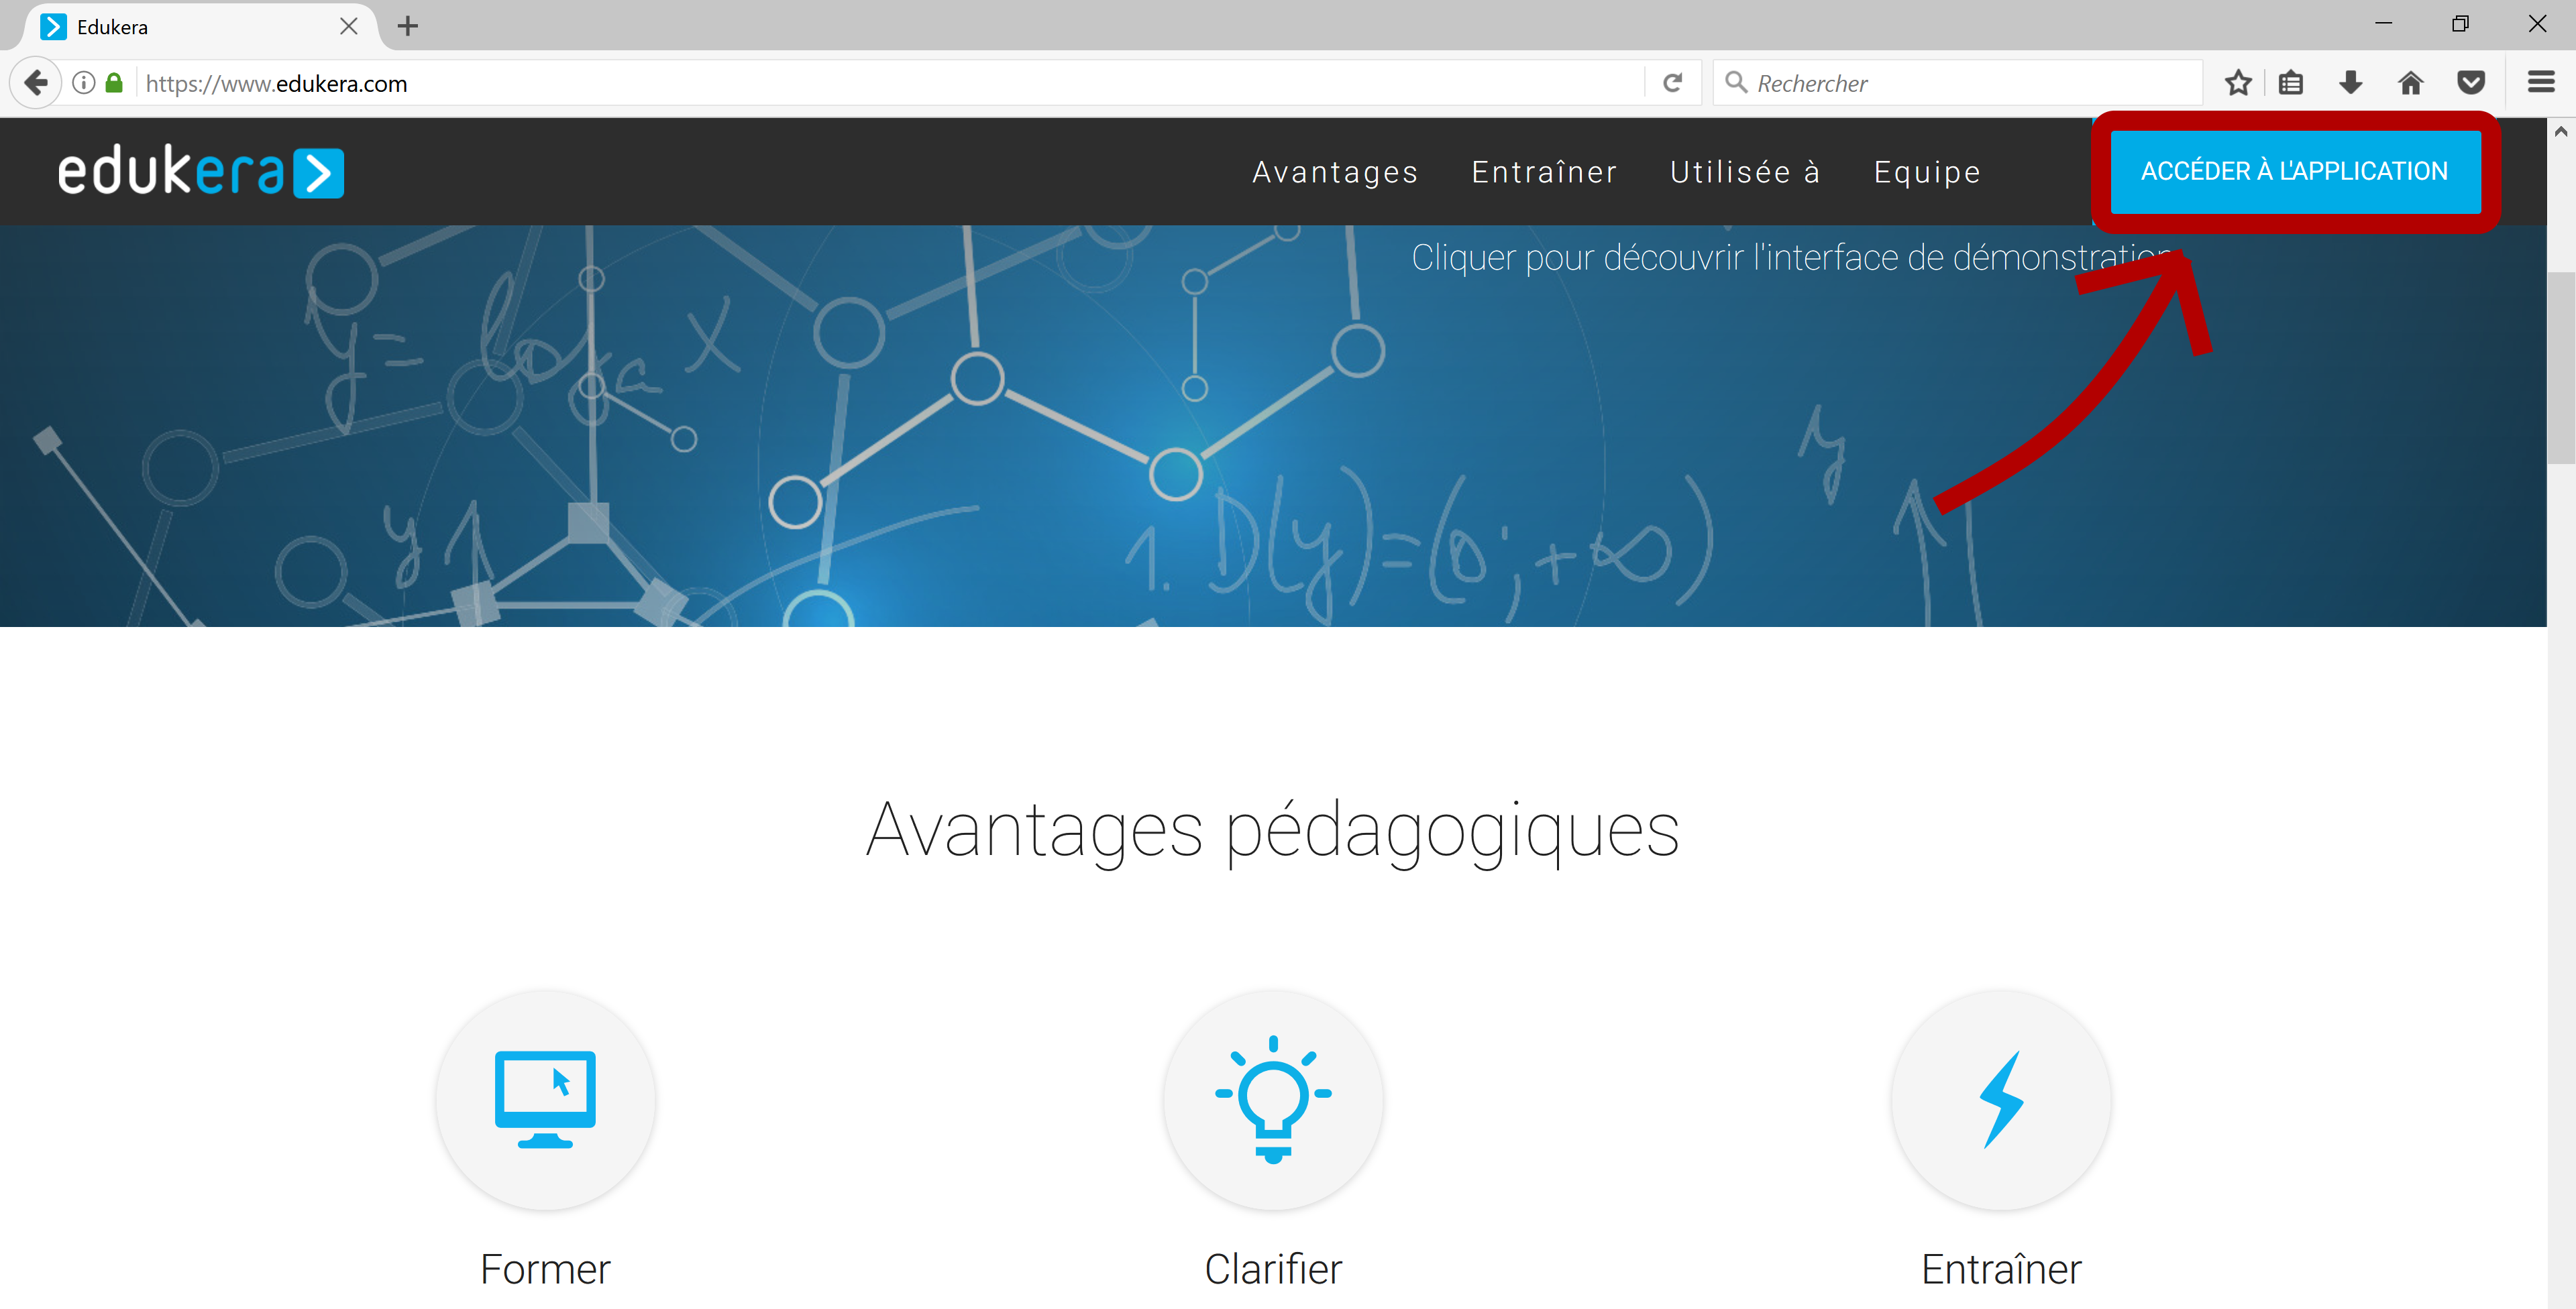
\includegraphics[scale=0.1]{img_site1.png}
\end{center}
\caption{Site Edukera}\label{im:site_edukera_bas}
\end{figure}
\FloatBarrier

Un nouvel onglet va s'ouvrir (l'adresse devrait être \url{https://app.edukera.com/}). Vous serez amenés à créer un compte, faites-le. La page de création de compte devrait ressembler à cela:
\begin{figure}
\begin{center}
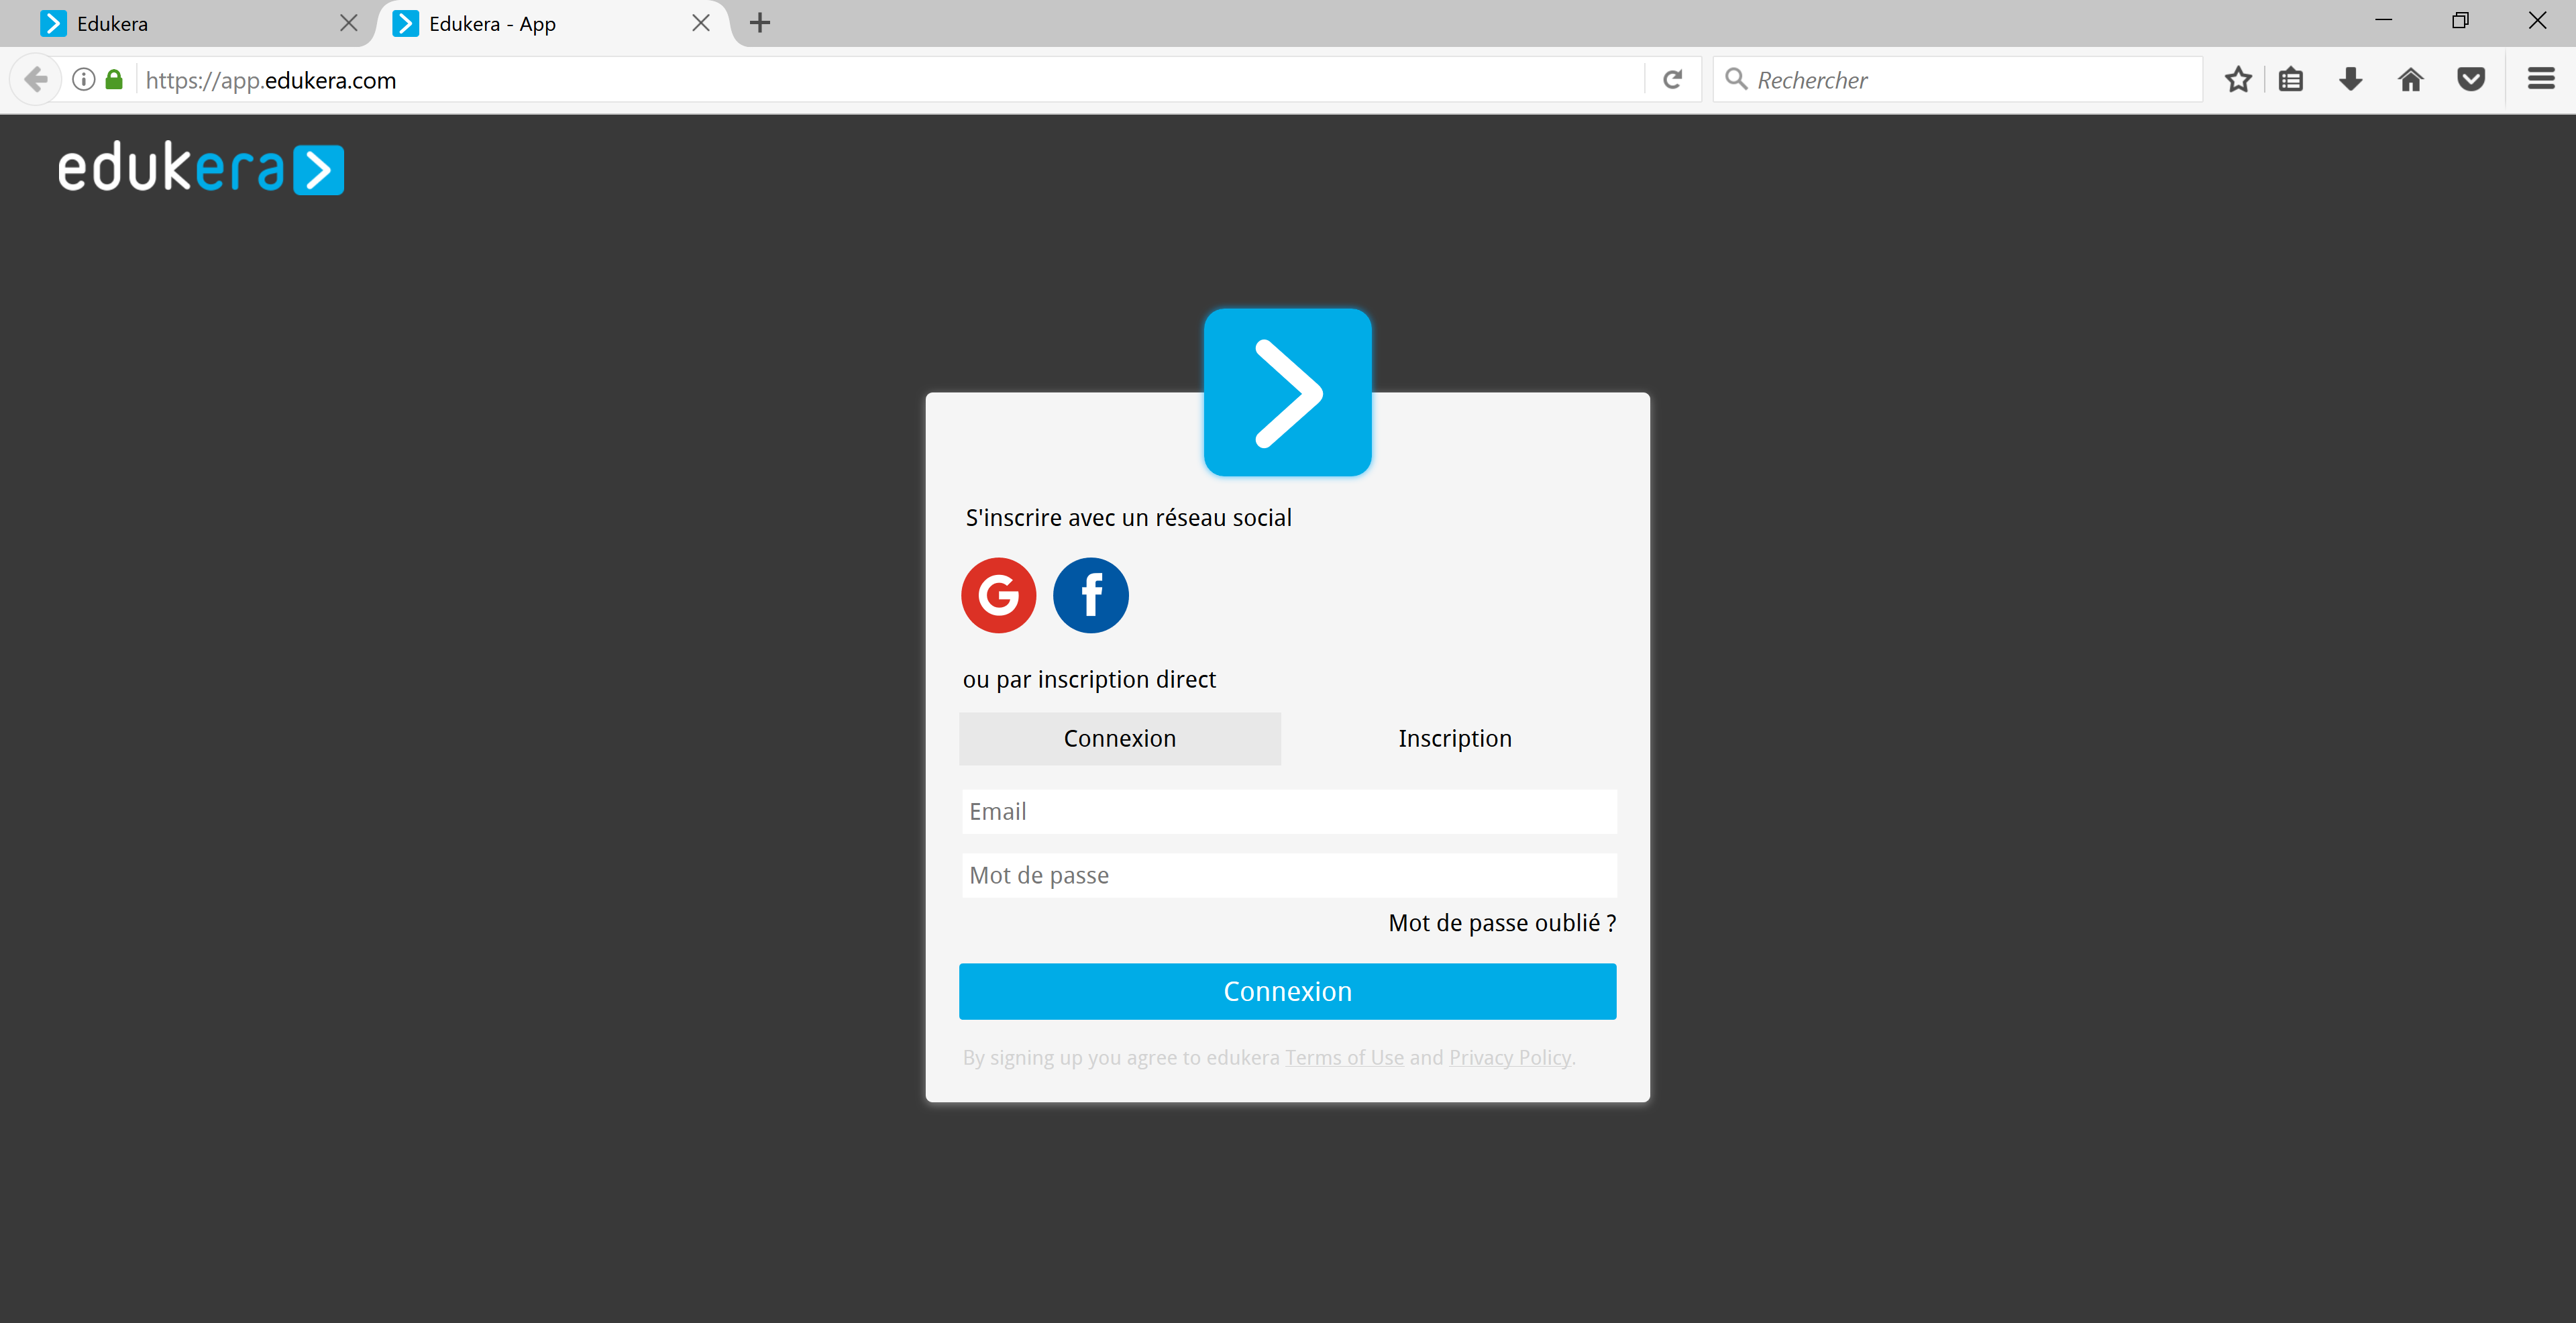
\includegraphics[scale=0.1]{img_app0.png}
\end{center}
\caption{Page de connexion / création du compte}\label{im:page_connexion}
\end{figure}
\FloatBarrier

Une nouvelle page se chargera ensuite, avec les option du compte (langue, e mail, mot de passe...)
Une fois que vos options vous conviennent, retournez à l'accueil, grâce au bouton en haut à gauche:
\begin{figure}[h!]
\begin{center}
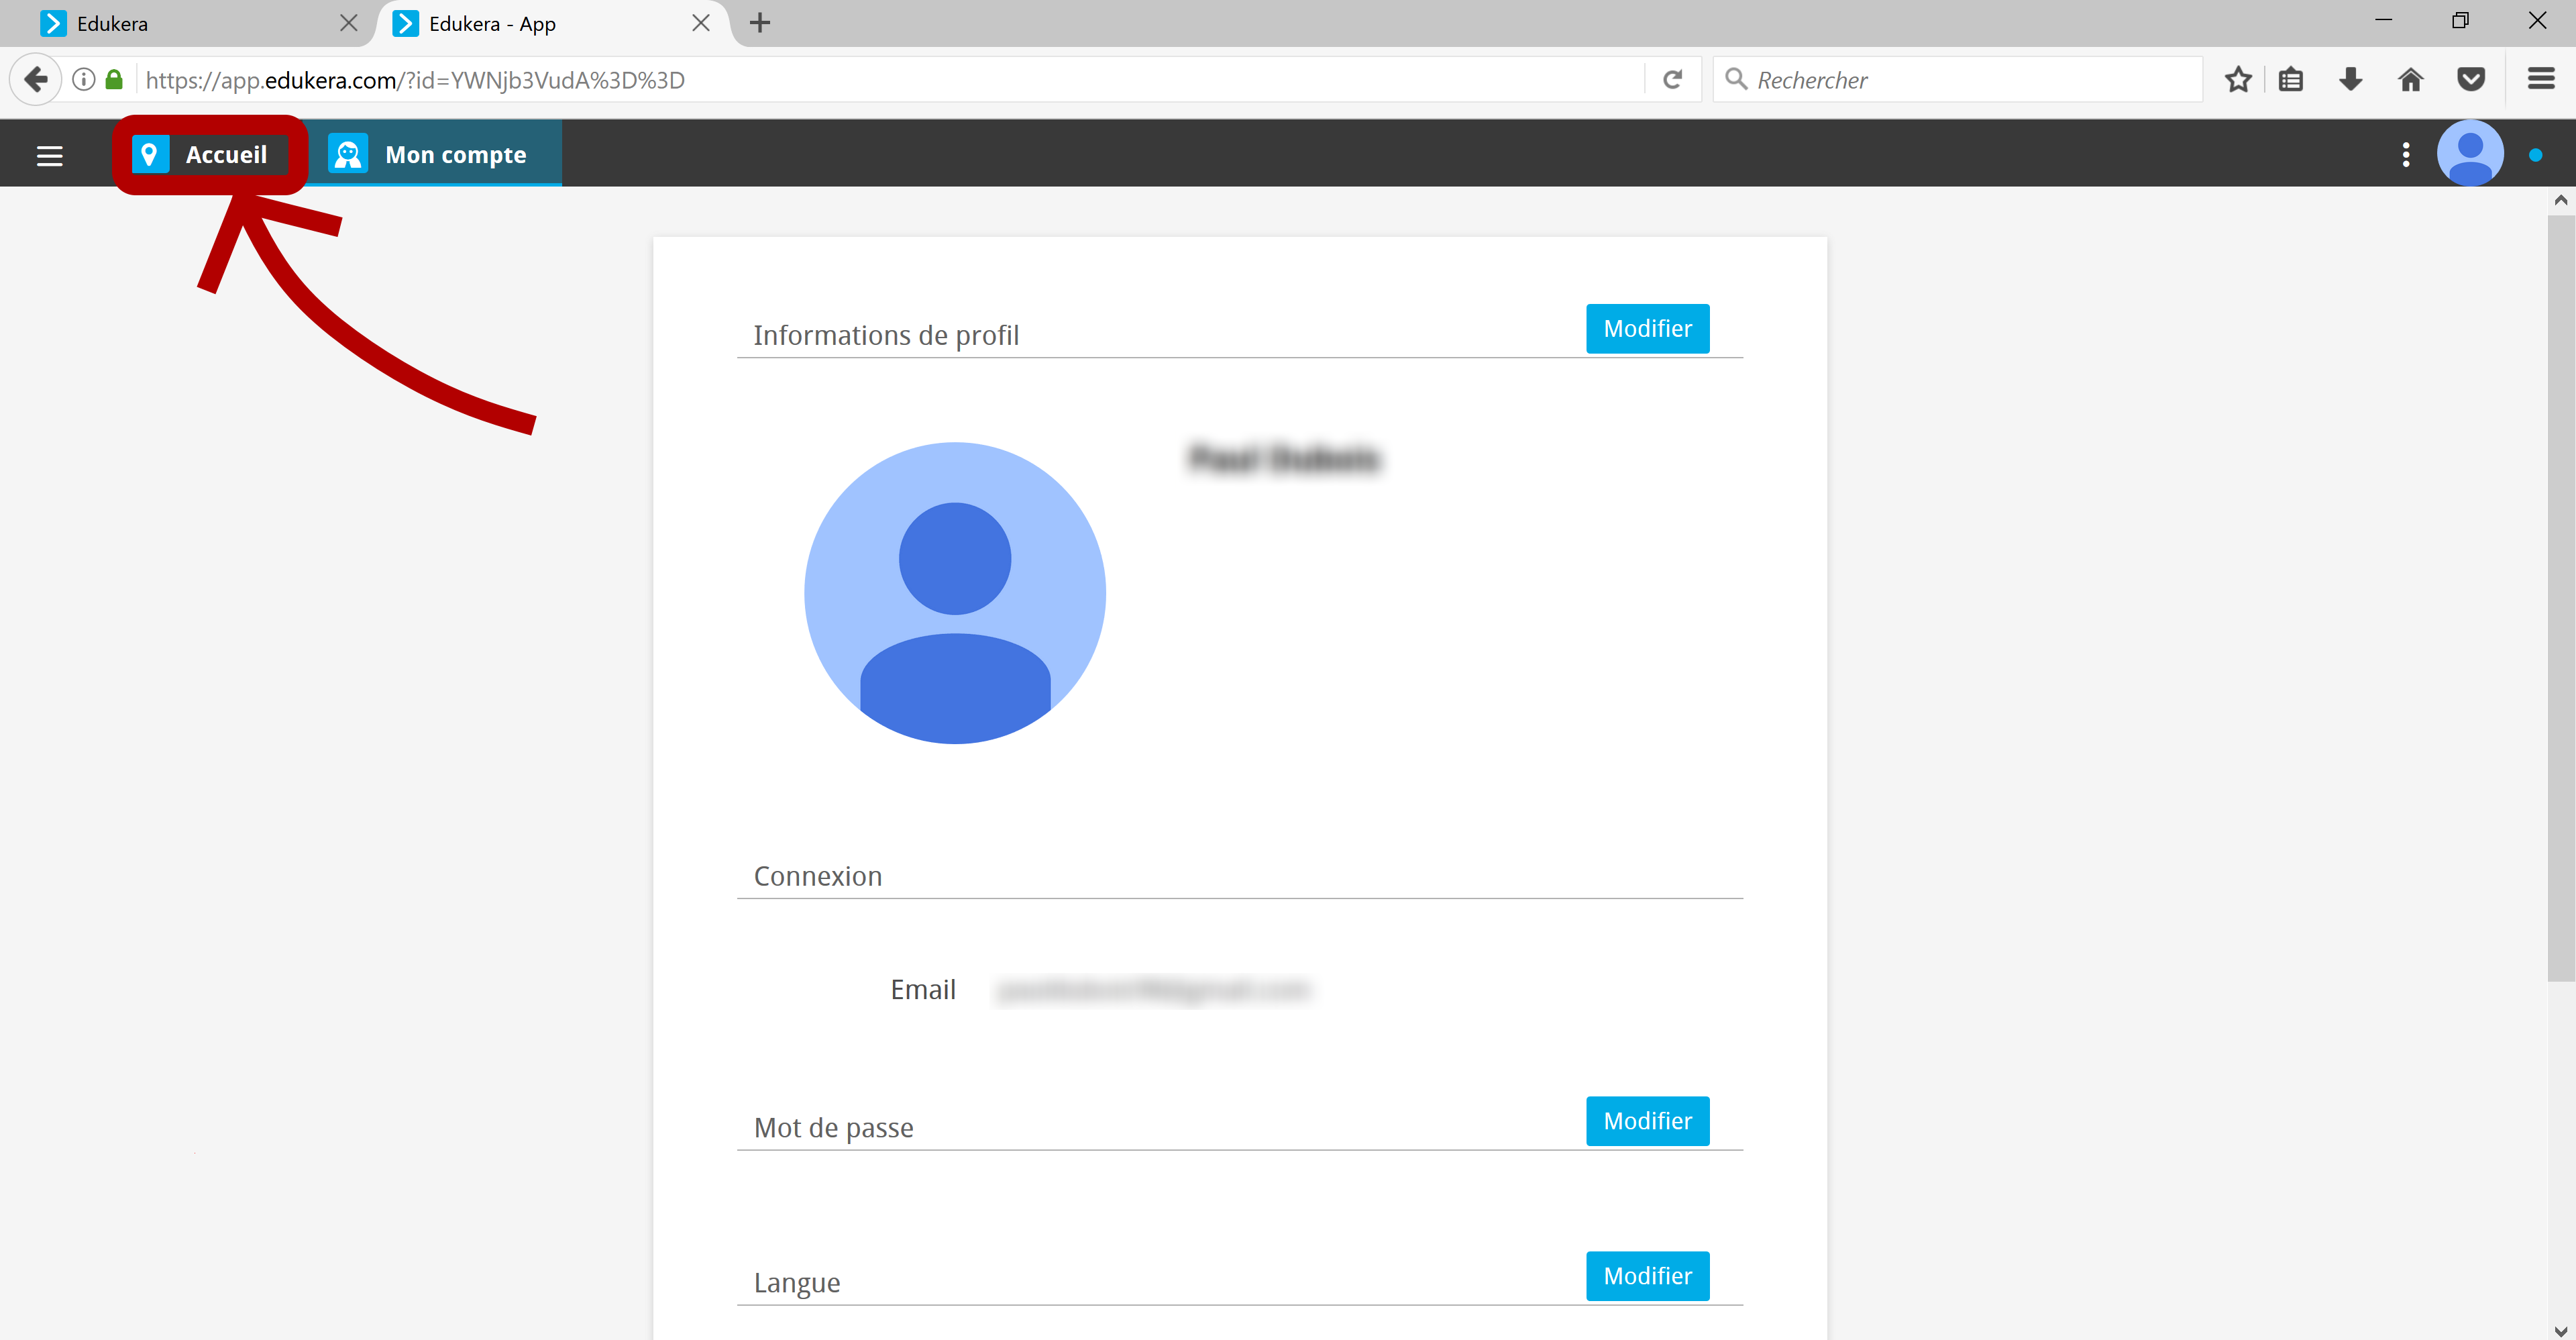
\includegraphics[scale=0.1]{img_app1.png}
\end{center}
\caption{Profile de l'utilisateur}\label{im:profile_utilisateur}
\end{figure}
\FloatBarrier



\section{Accéder aux exercices}



Le site propose 4 sujets: Logique, Calcul algébrique, Analyse, et Ensembles
Au départ, il est vivement conseillé de faire les exercices de logique (les autres domaines viendront plus tard, car ils sont plus complexes).
Cliquez donc sur le bouton "commencer" associé à la partie logique.
\begin{figure}[h!]
\begin{center}
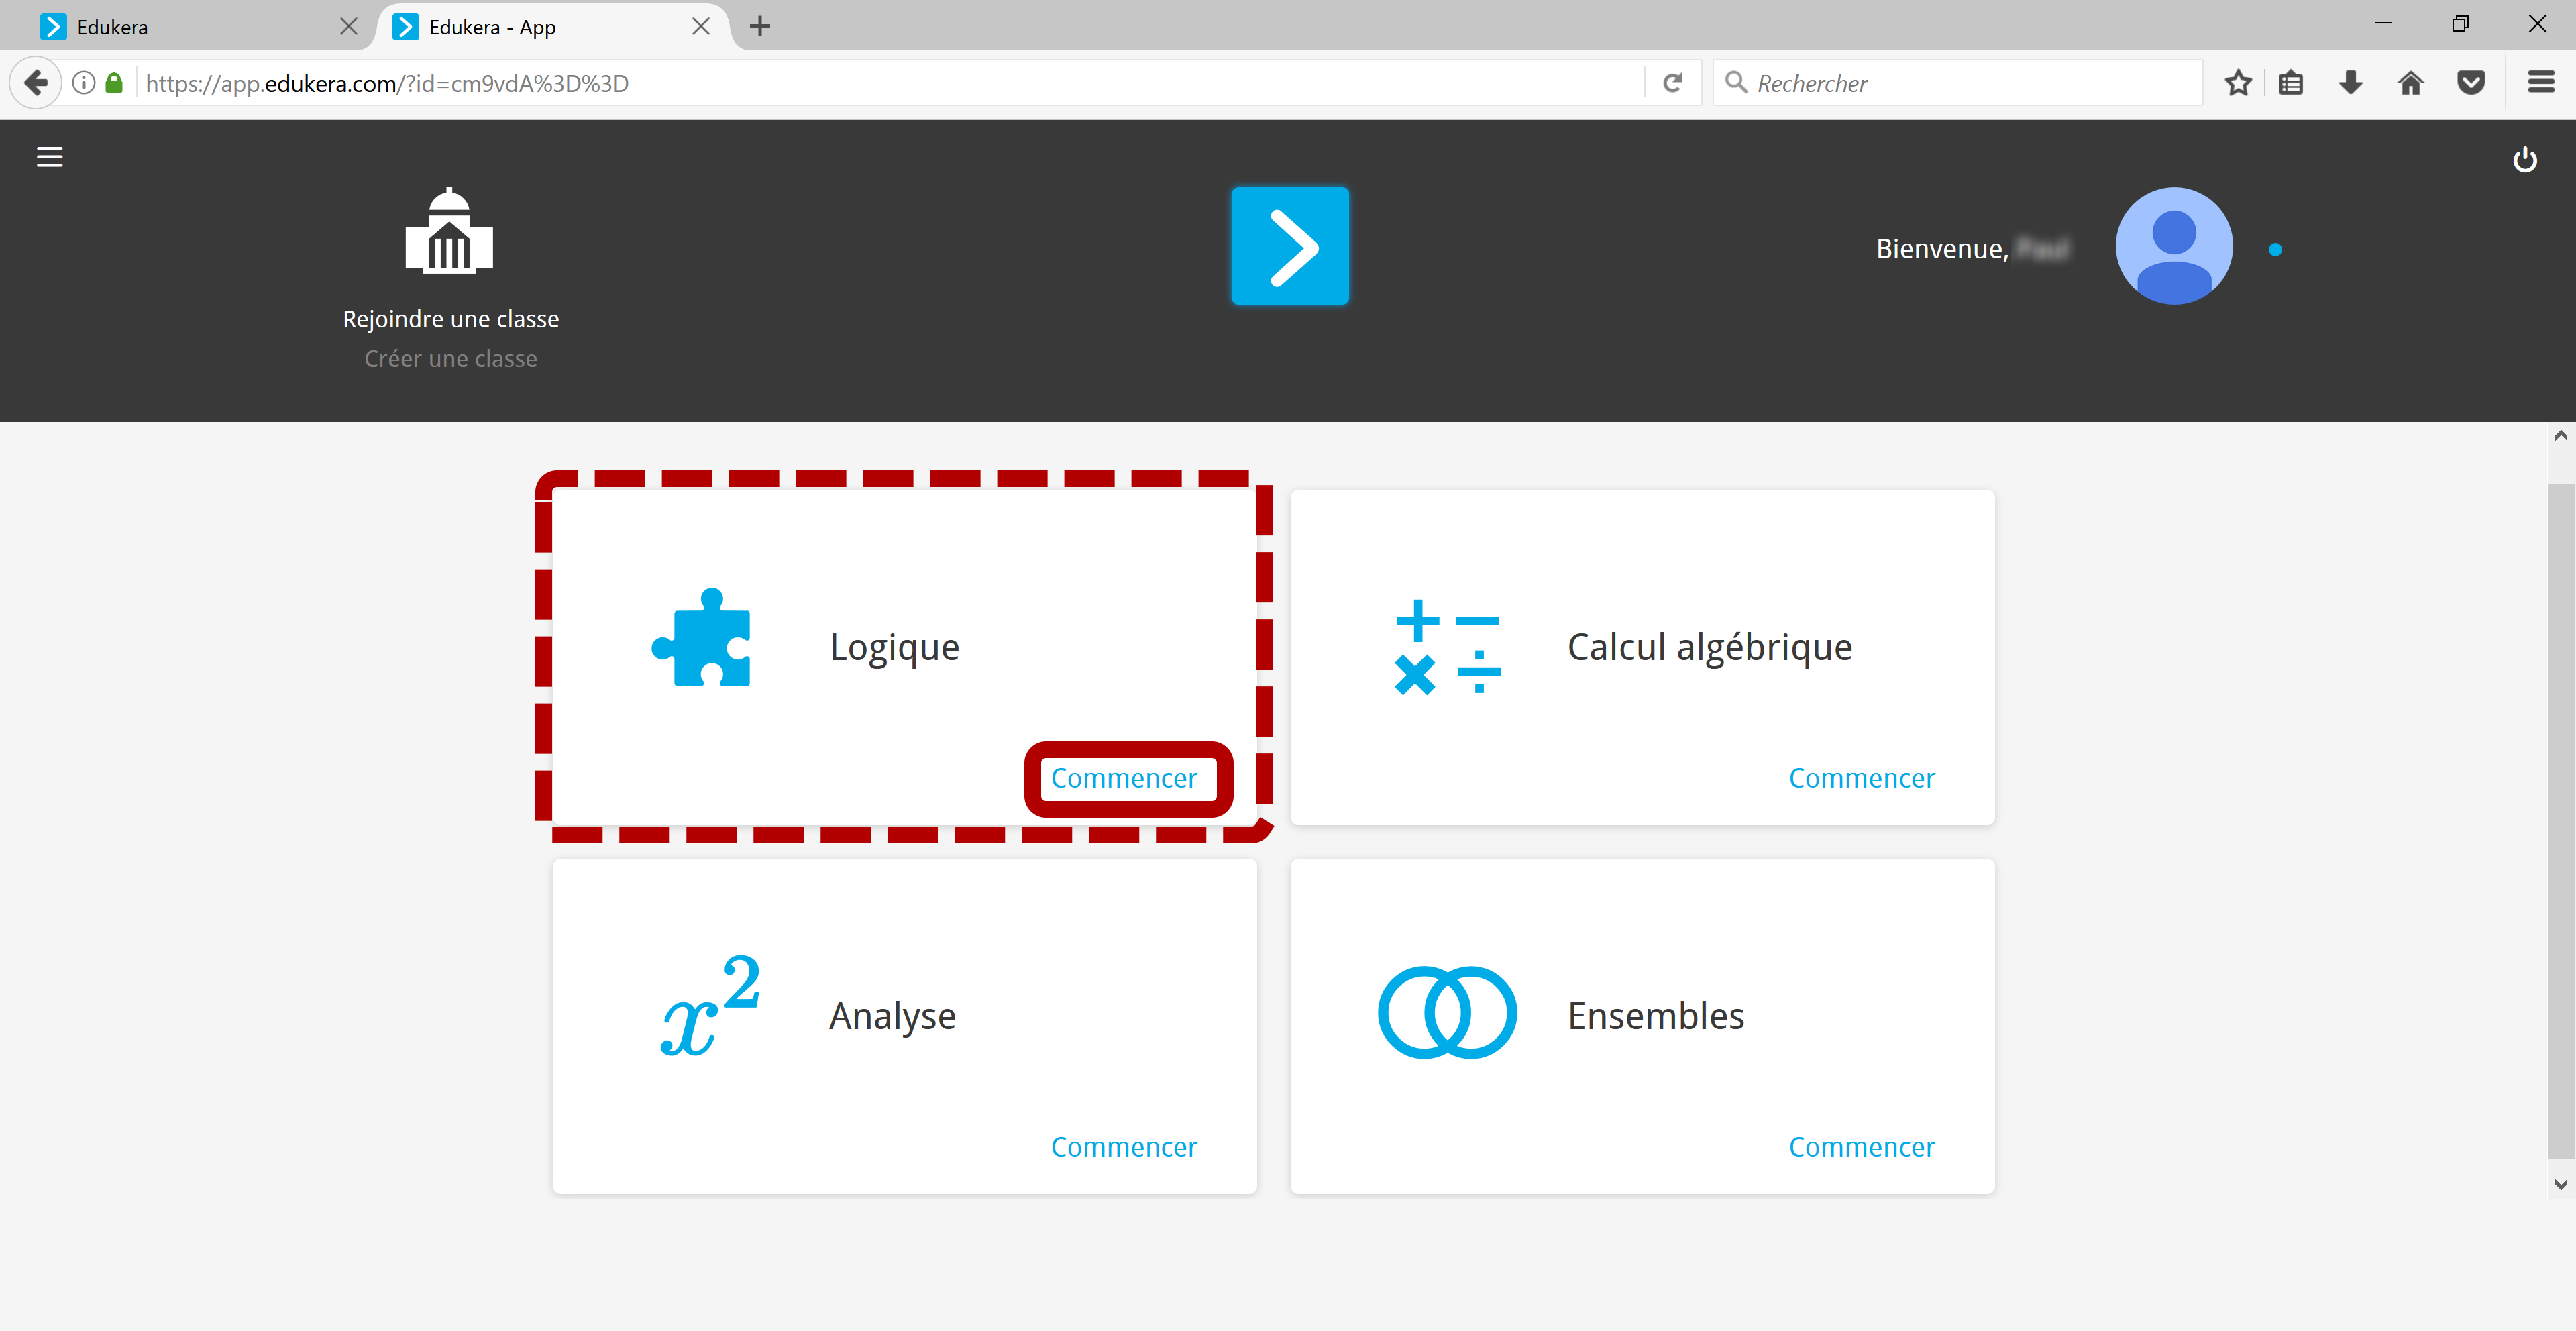
\includegraphics[scale=0.1]{img_app2.png}
\end{center}
\caption{Écran d'accueil de l'application}\label{im:accueil}
\end{figure}
\FloatBarrier

Vous arriverez sur une nouvelle page, vous demandant de faire un nouveau choix: Connecteurs ou quantificateurs.
Là encore, il est conseillé de commencer par les connecteurs.
\begin{figure}[h!]
\begin{center}
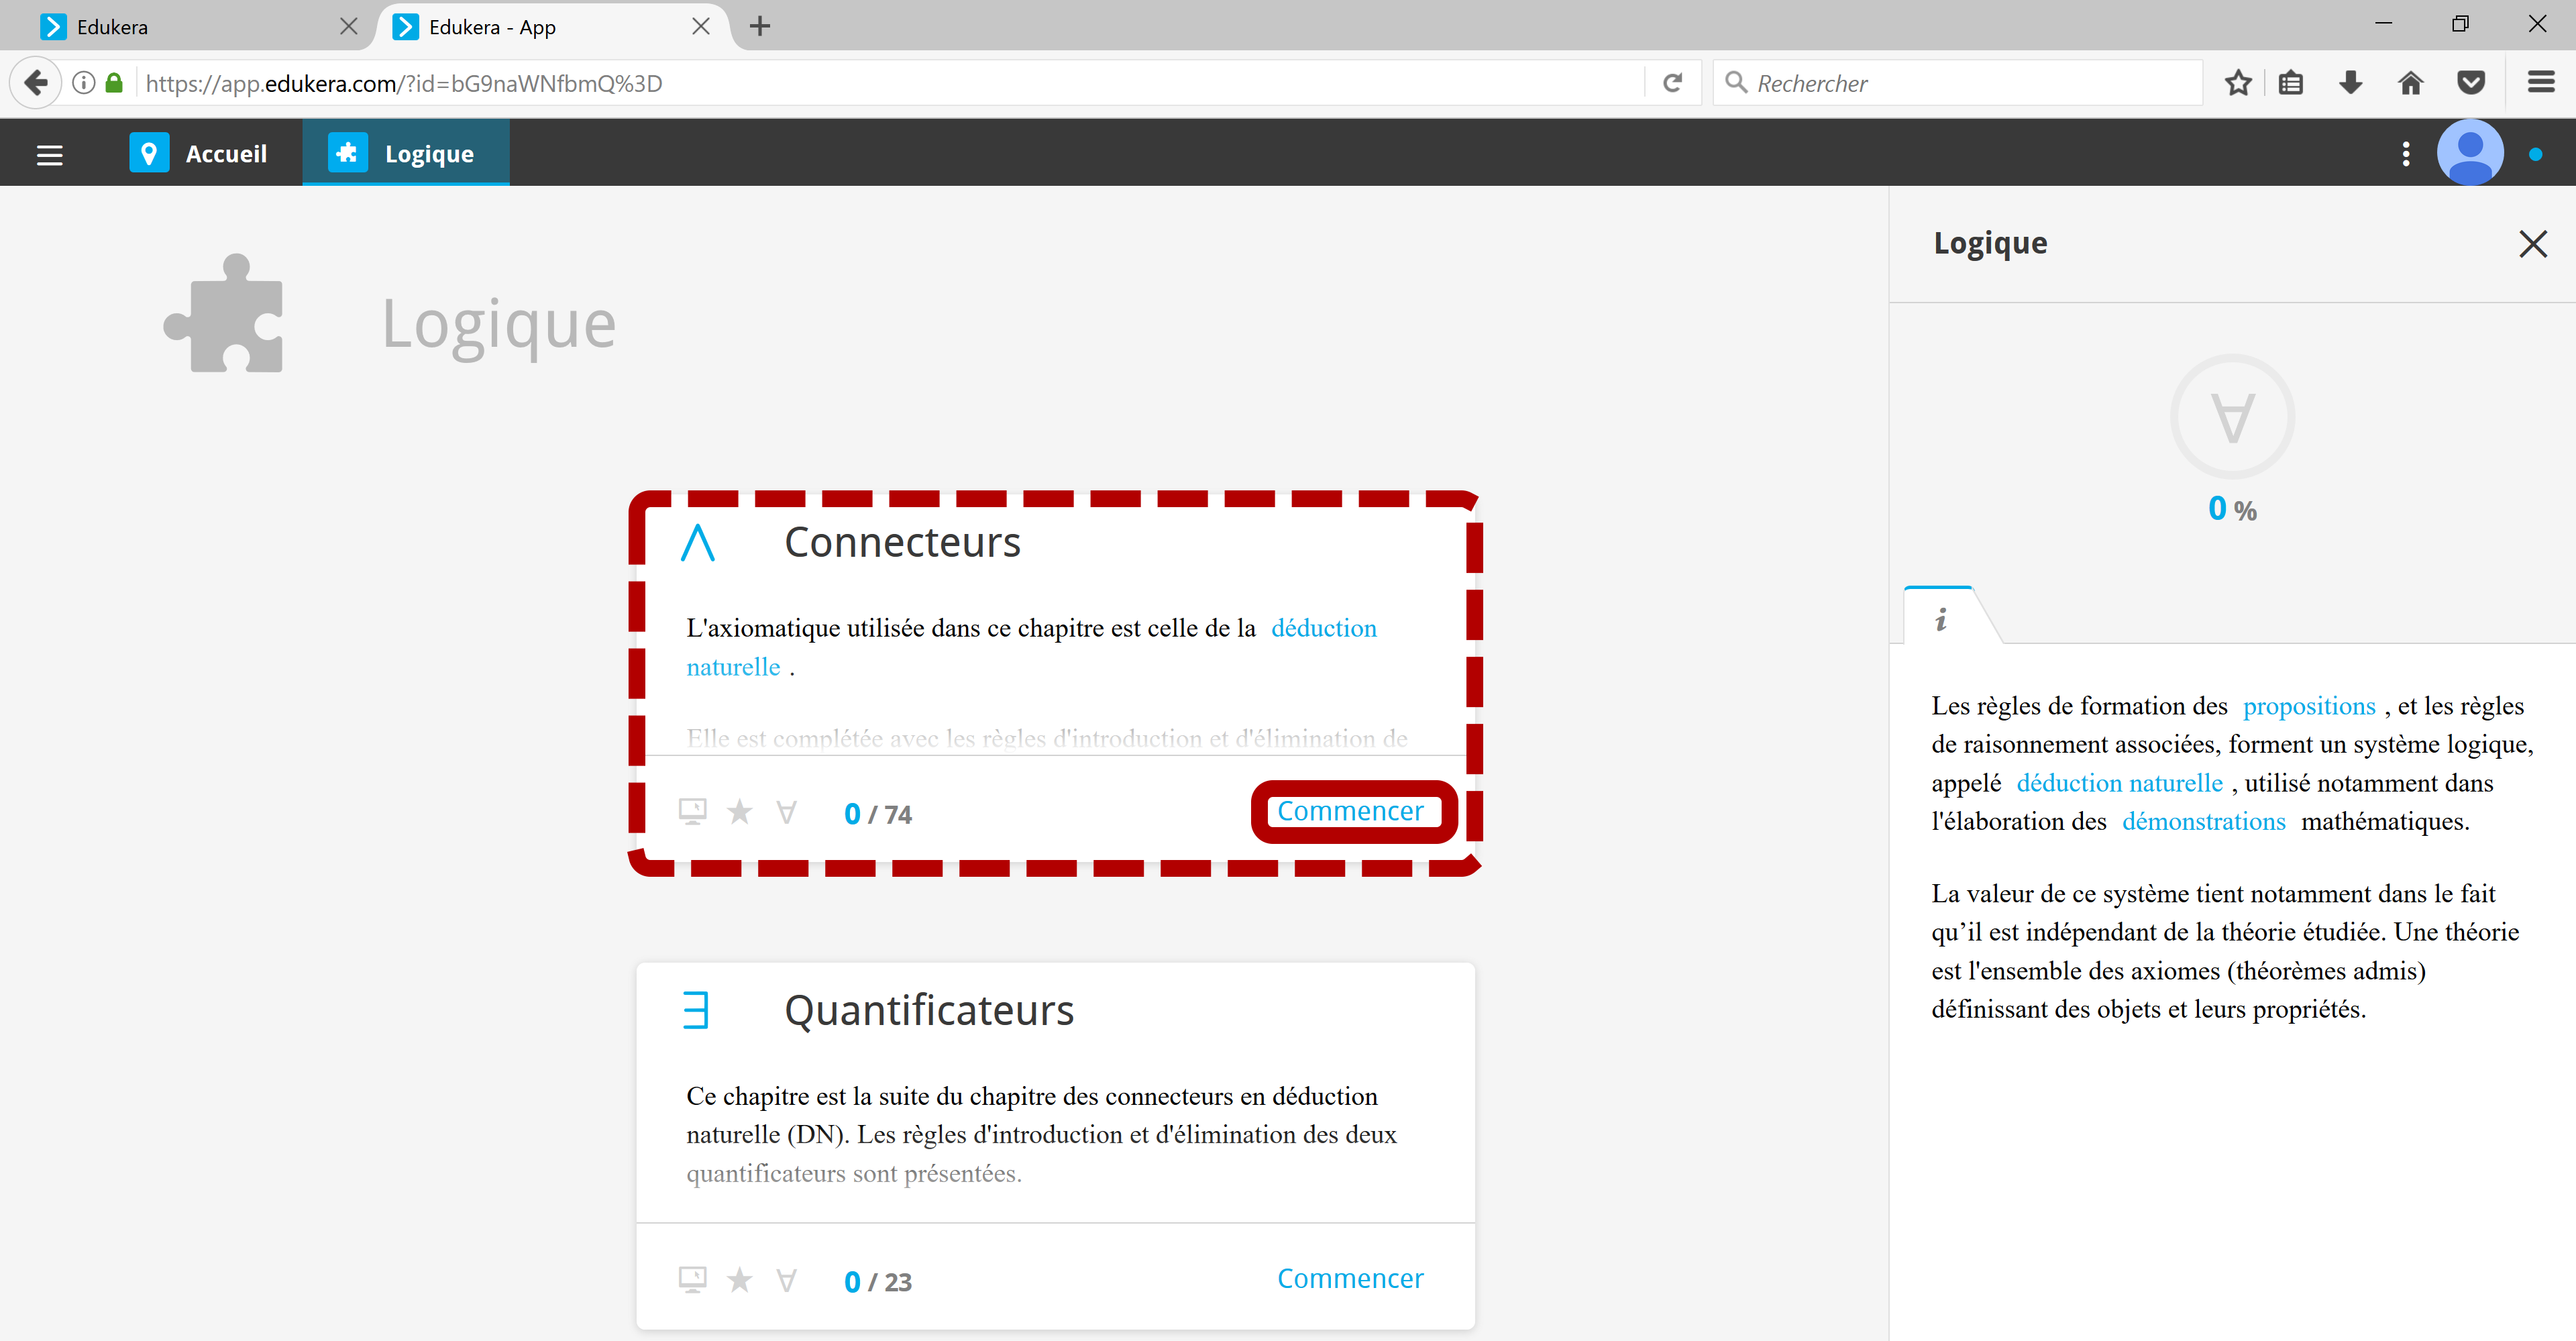
\includegraphics[scale=0.1]{img_app3.png}
\end{center}
\caption{Accueil de la partie "logique"}\label{im:logique_accueil}
\end{figure}
\FloatBarrier

On vous affiche alors la liste des exercices, le premier est guidé. 
\begin{figure}[h!]
\begin{center}
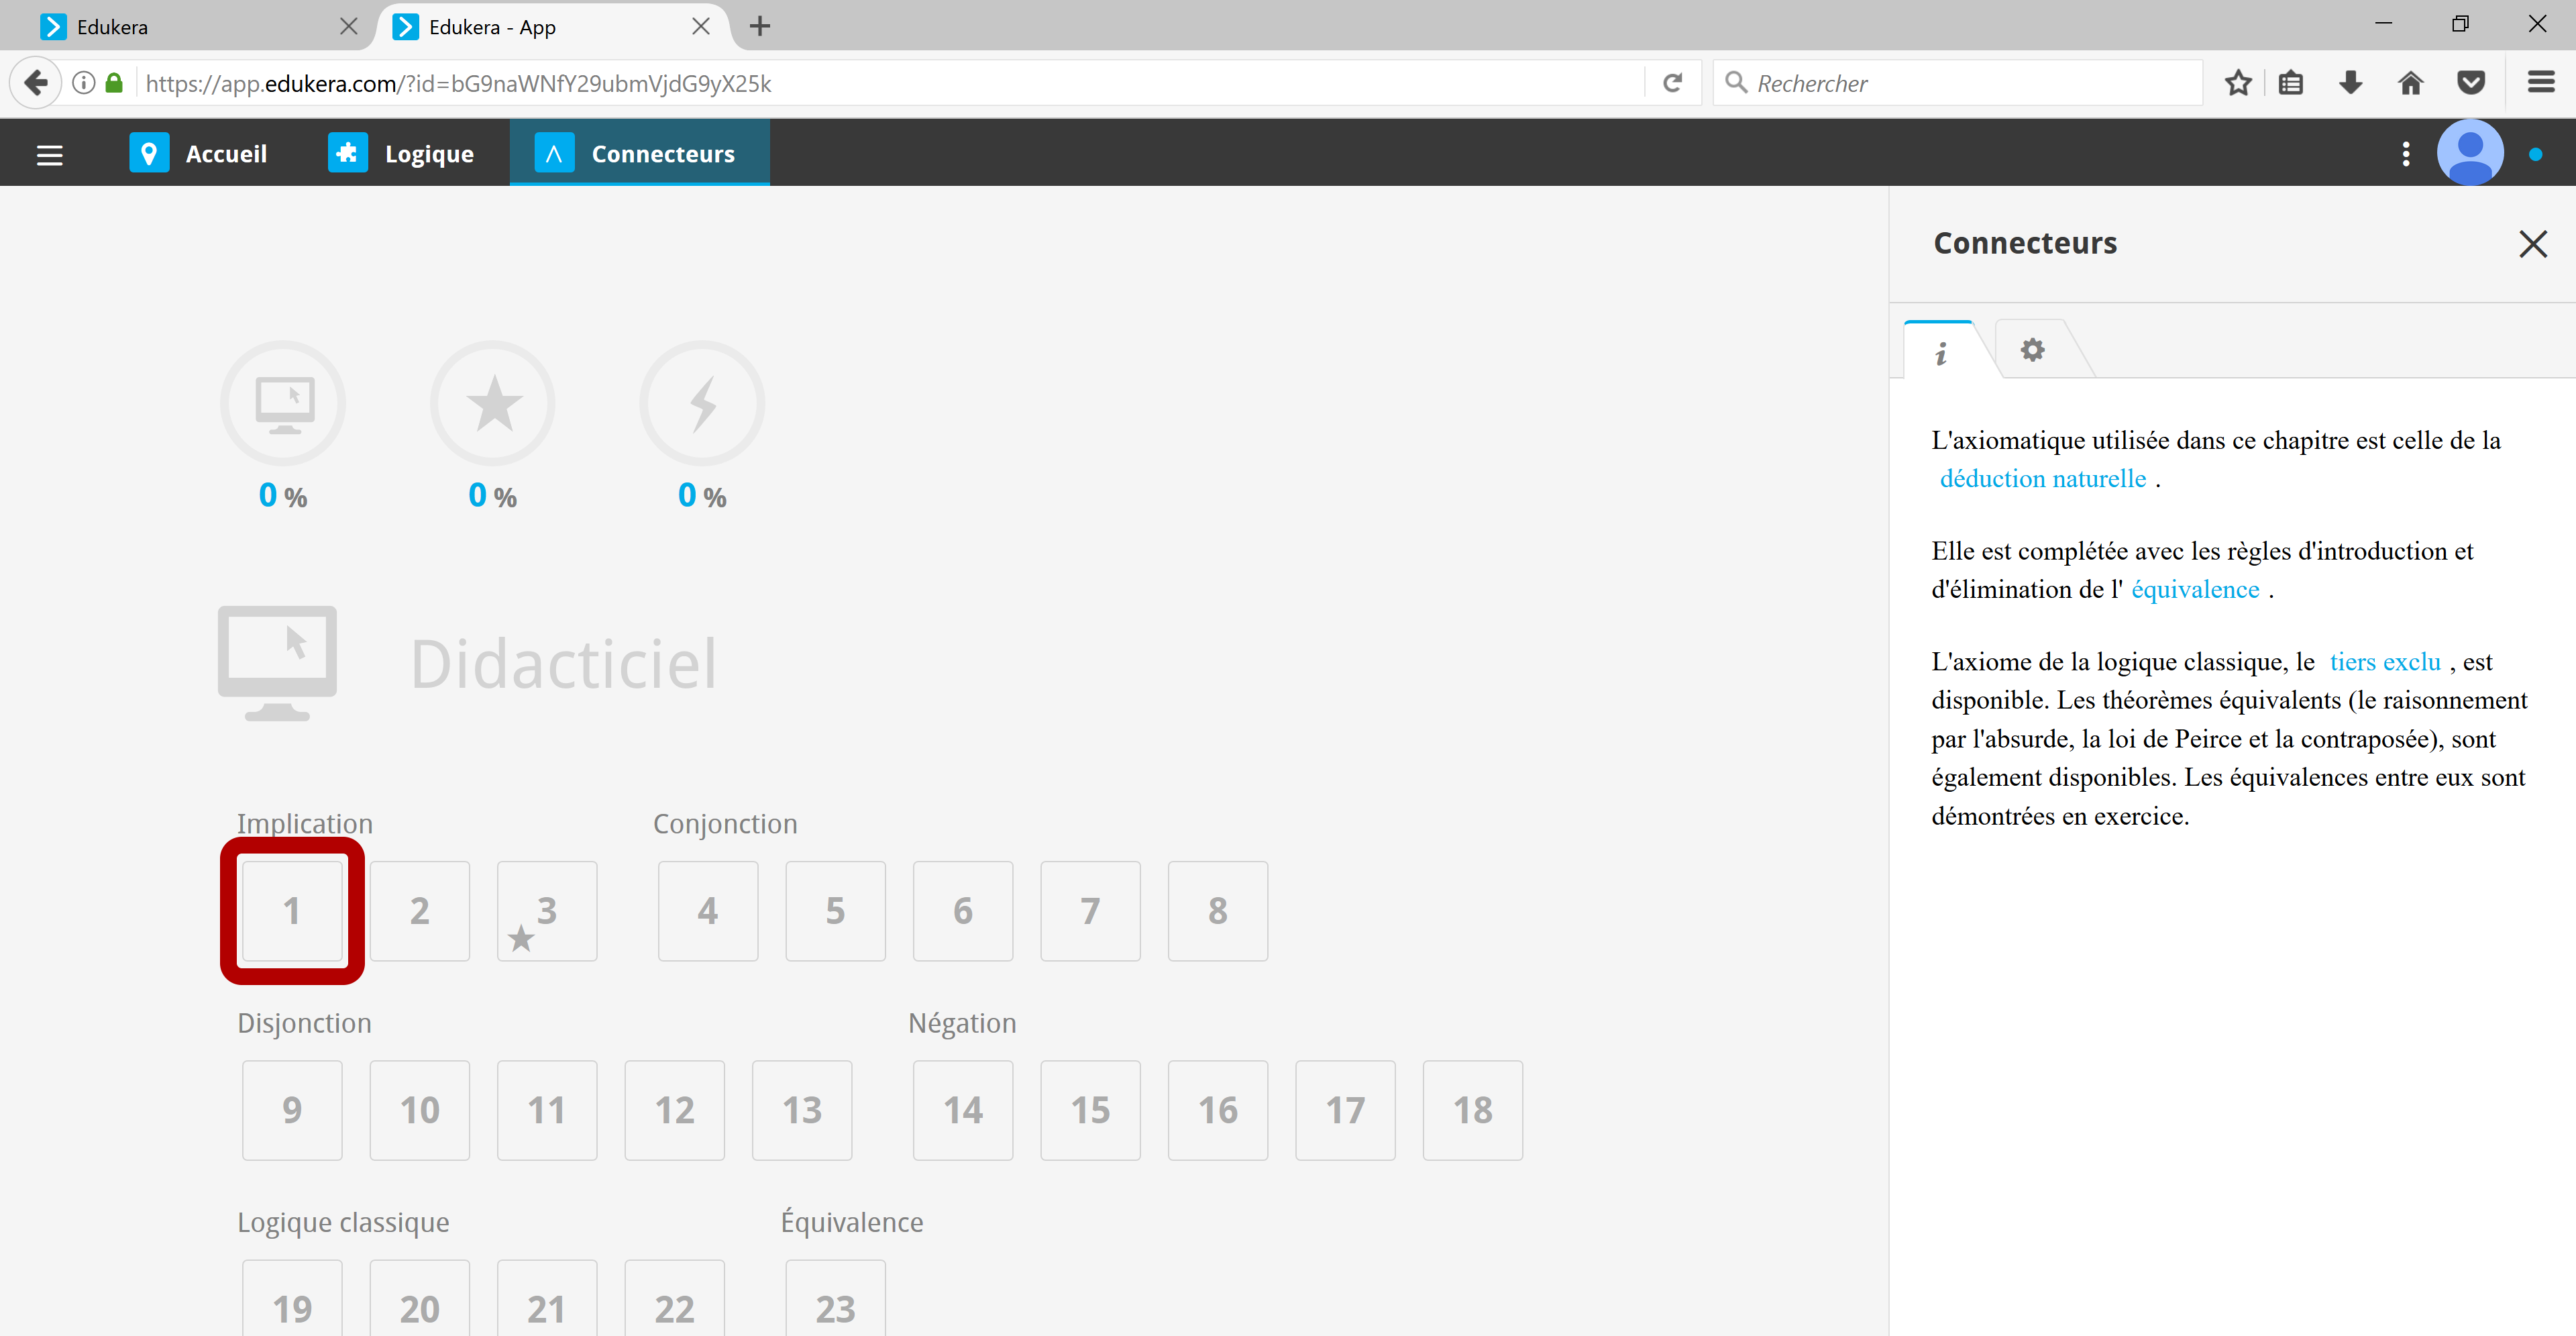
\includegraphics[scale=0.1]{img_app4.png}
\end{center}
\caption{Accueil de la partie "connecteurs"}\label{im:connecteurs_accueil}
\end{figure}
\FloatBarrier

Si vous suivez les explications, il ne devrait pas y avoir de problème (il faut cliquer sur suivant, ou bien sur les boutons de l'interface qui sont mis en valeur).
Je fais tout de même un petit résumé graphique:
\begin{figure}[h!]
\begin{center}
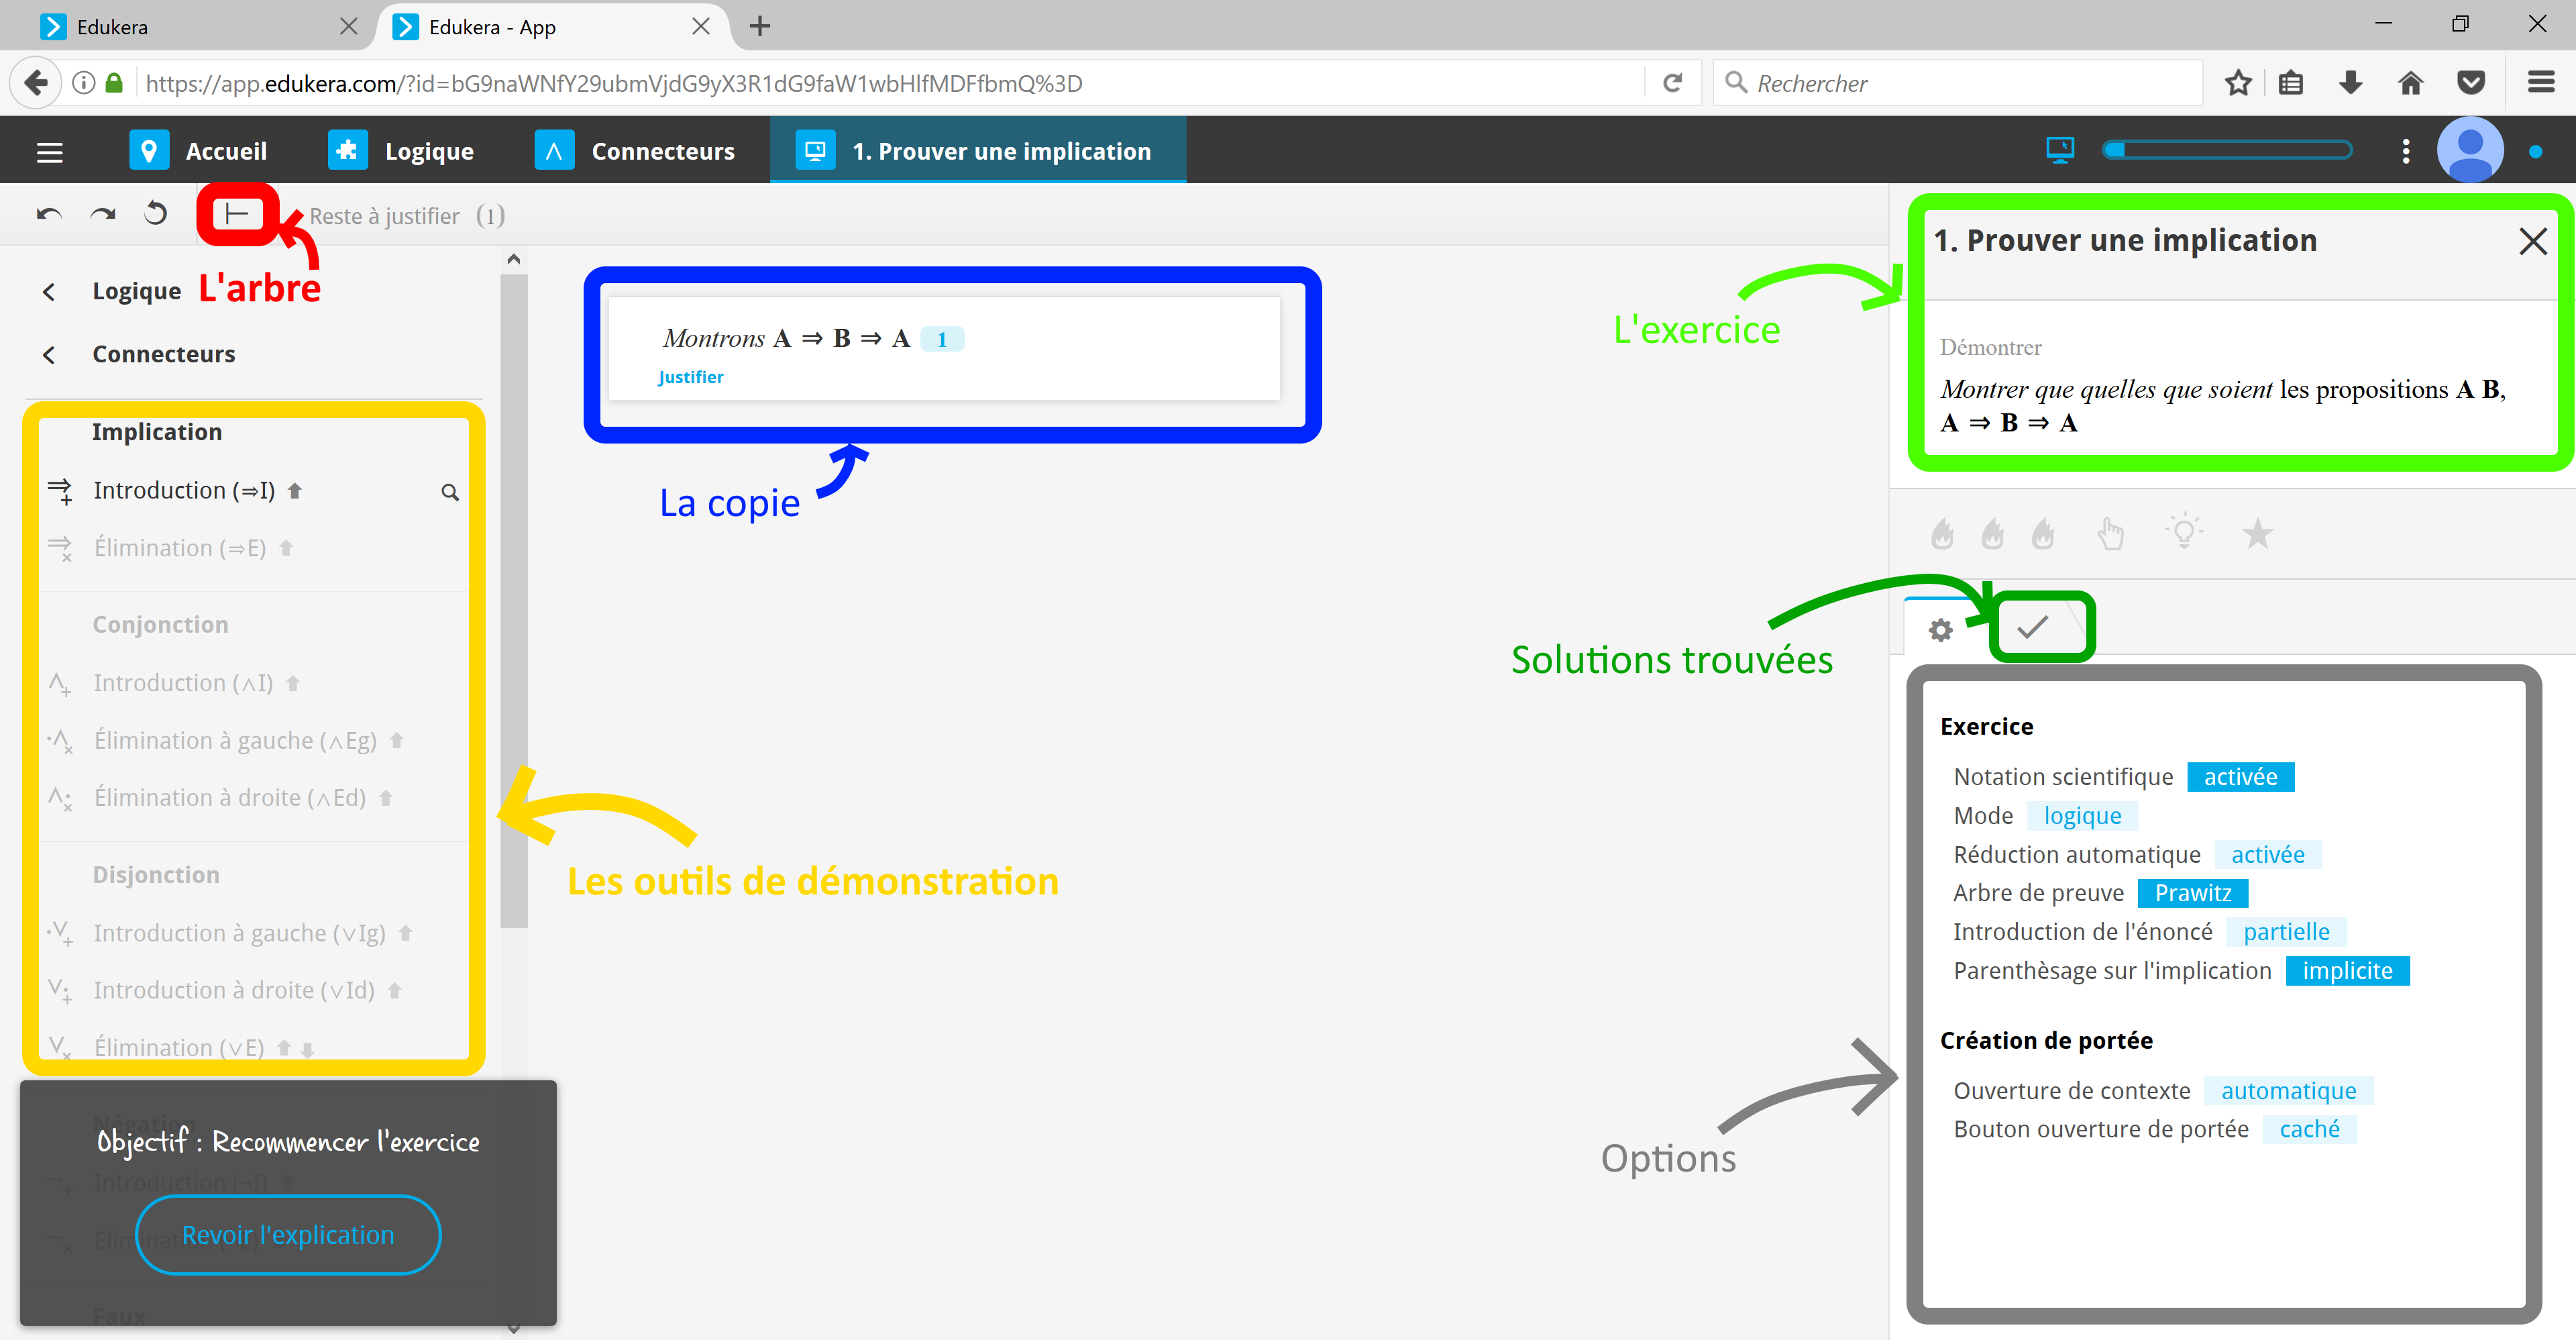
\includegraphics[scale=0.1]{img_app5.png}
\end{center}
\caption{Interface de déonstration}\label{im:interface_demo}
\end{figure}
\FloatBarrier

La copie n'étant pas forcément très parlant au départ, je conseille d'afficher l'arbre (le bouton est en haut à gauche). A noter que deux affichages sont disponibles pour l'arbre: "Prawitz" et "séquent". Vous pouvez basculer de l'un à l'autre dans les options (bandeau de droite).

Dans les premiers exercices, vous découvrirez les outils de démonstration (introduction/élimination d'une implication...). Il est donc normal que tous ne soient pas disponibles dès le départ.

Dans solutions trouvées, il y a un historique des solutions à l'exercice que vous avez trouver; Cela peut être intéressant si vous voulez trouver deux solutions différentes.

Lorsque vous aurez plusieurs propositions à justifier, sélectionnez la proposition avant d'y ajouter un bloc, si non, le bloc pourra être ajouté à une autre justification, ou bien ne sera pas ajouté.
\begin{figure}[h!]
\begin{center}
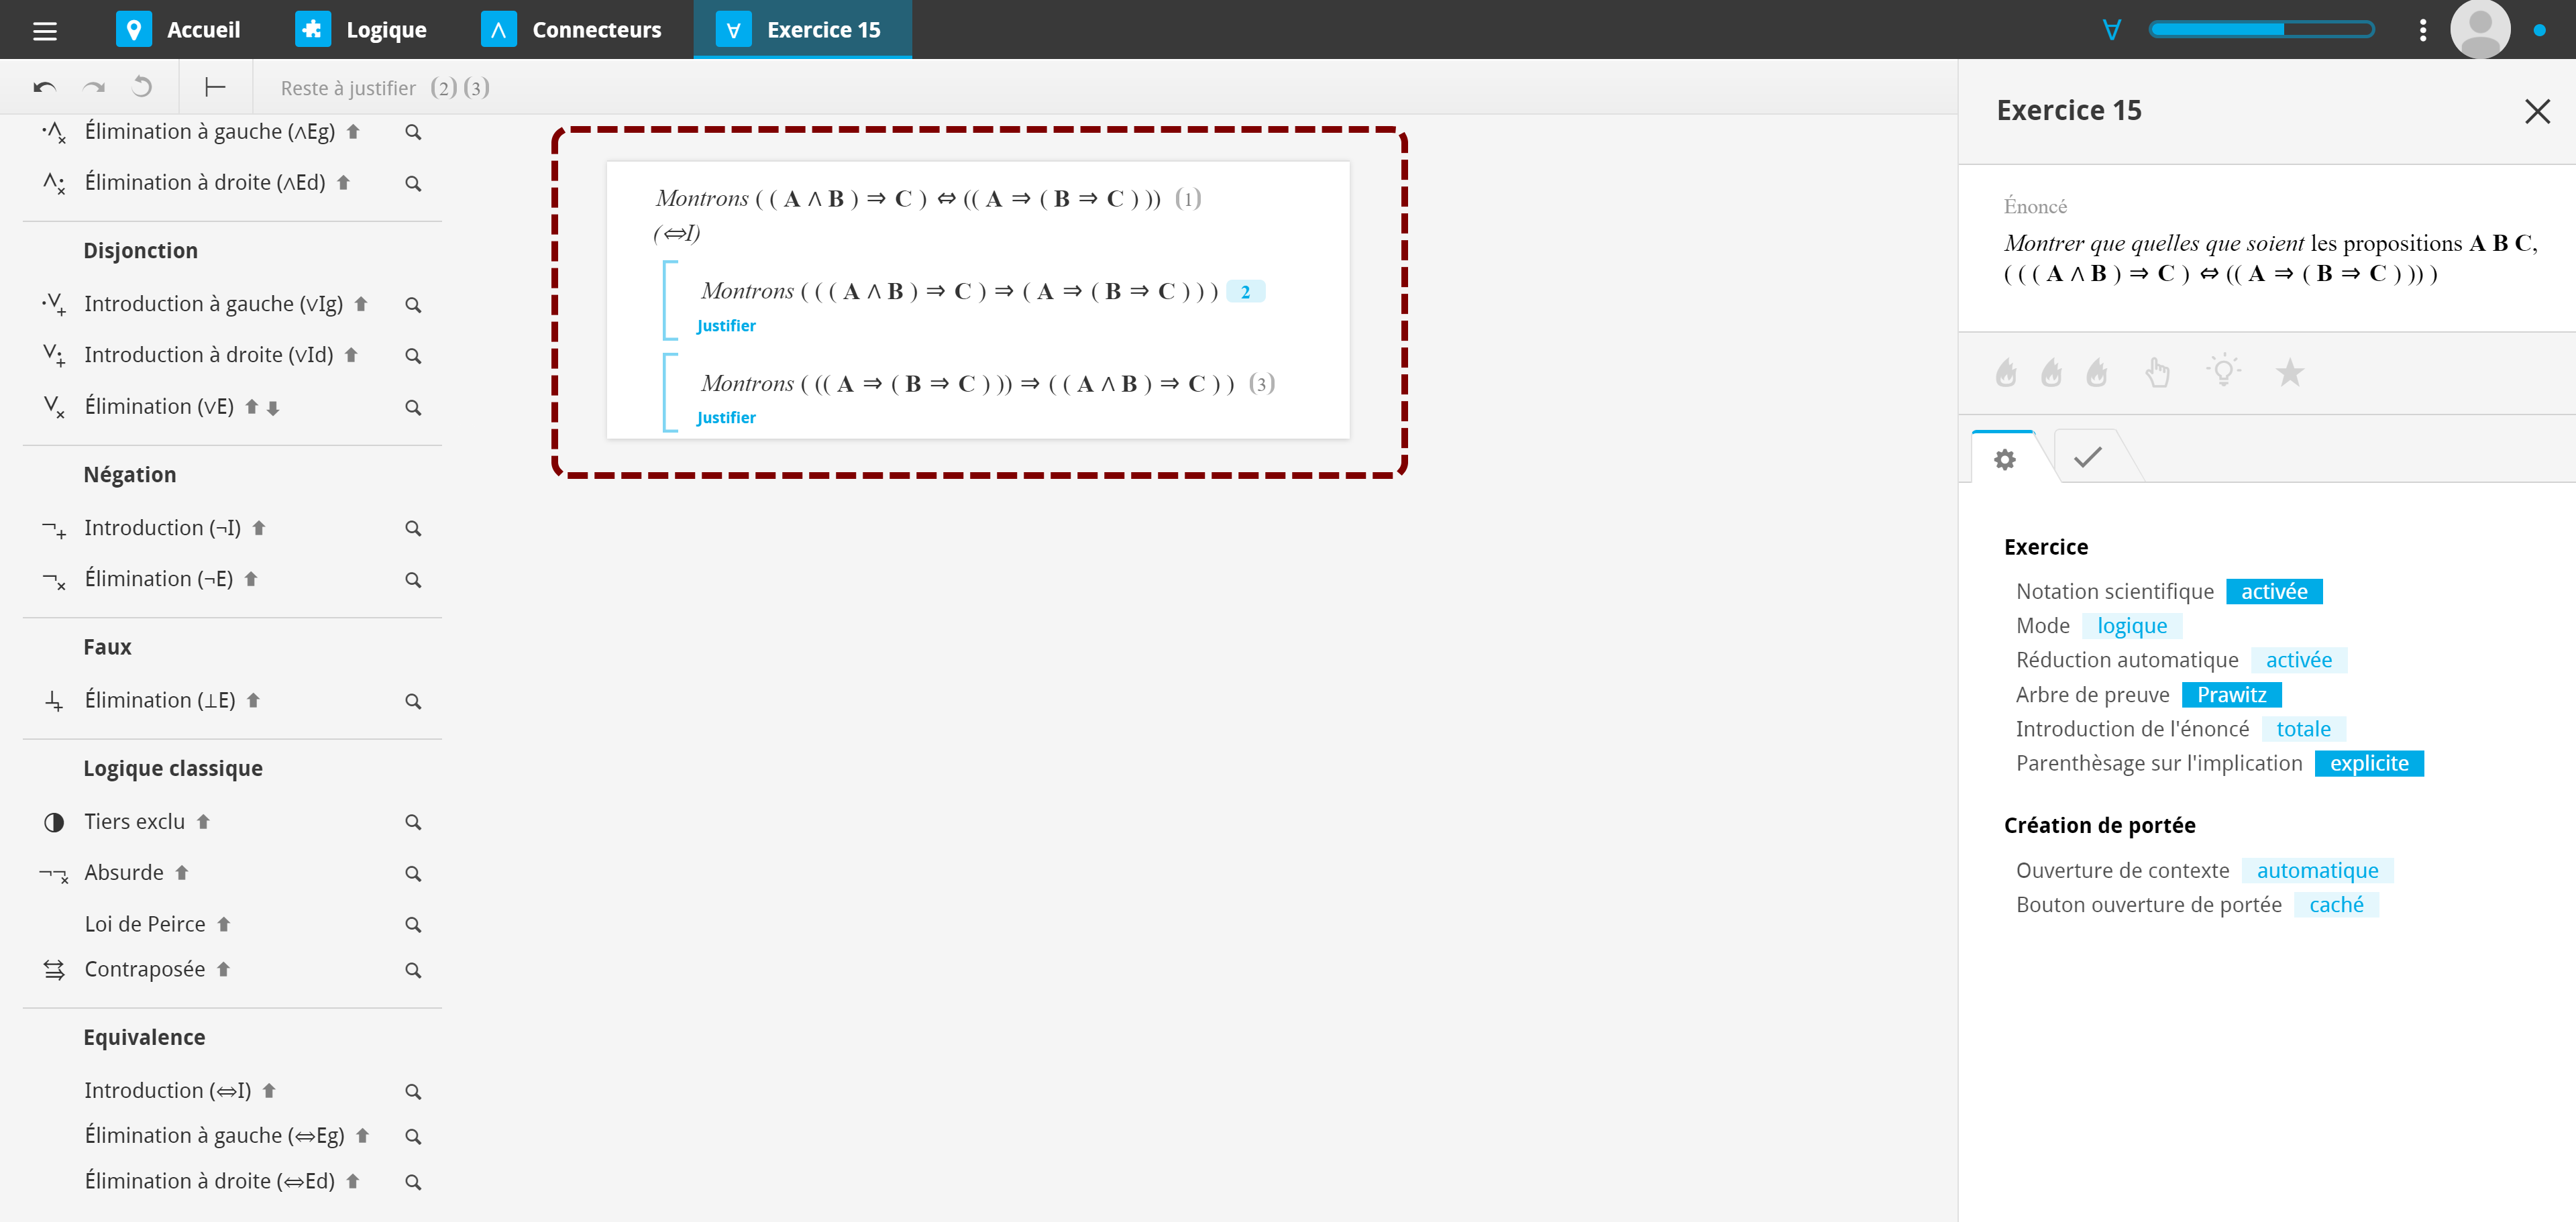
\includegraphics[scale=0.05]{img_app6.png}
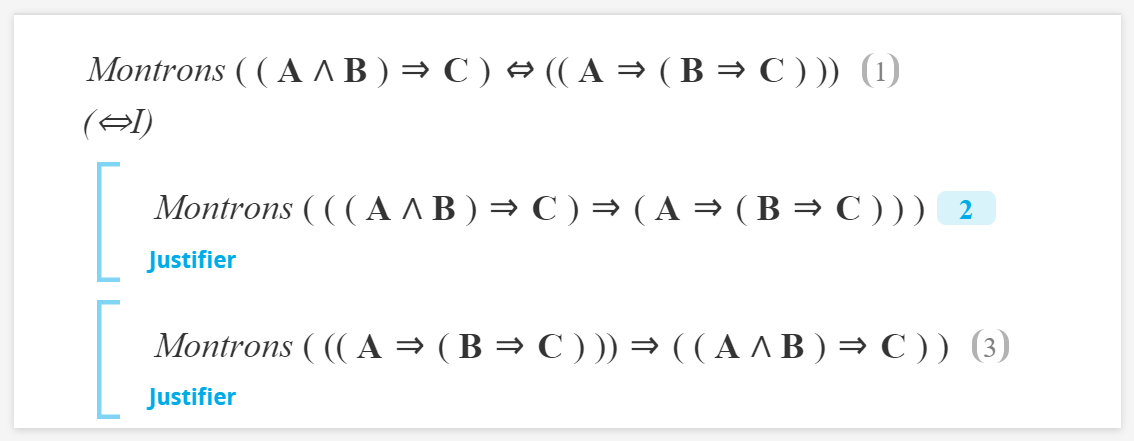
\includegraphics[scale=0.16]{img_app7.png}
\end{center}
\caption{Sélection des propositions}\label{im:selec_prop}
\end{figure}
\FloatBarrier

Ici, la proposition 2 est sélectionnée (le numéro est encadré de bleu clair), si vous ajoutez des blocs de justifications, ce sera sur cette proposition.
Pour changer la proposition sélectionnée, cliquez dessus.

Vous remarquerez certainement que certains blocs peuvent être appliqués tout le temps, alors que d'autres peuvent rendre la proposition impossible à justifier.
Je m'explique: si vous devez justifier A \textit{et} B, alors vous pouvez introduire un '\textit{et}', c'est-à-dire justifier A et B séparément.
Par contre, si vous devez justifier A \textit{ou} B, alors introduire un '\textit{ou}' (menant à justifier seulement A, par exemple) peut rendre la proposition impossible à justifier.

Une image vaut mieux qu'une longue explication:
\begin{figure}[h!]
\begin{center}
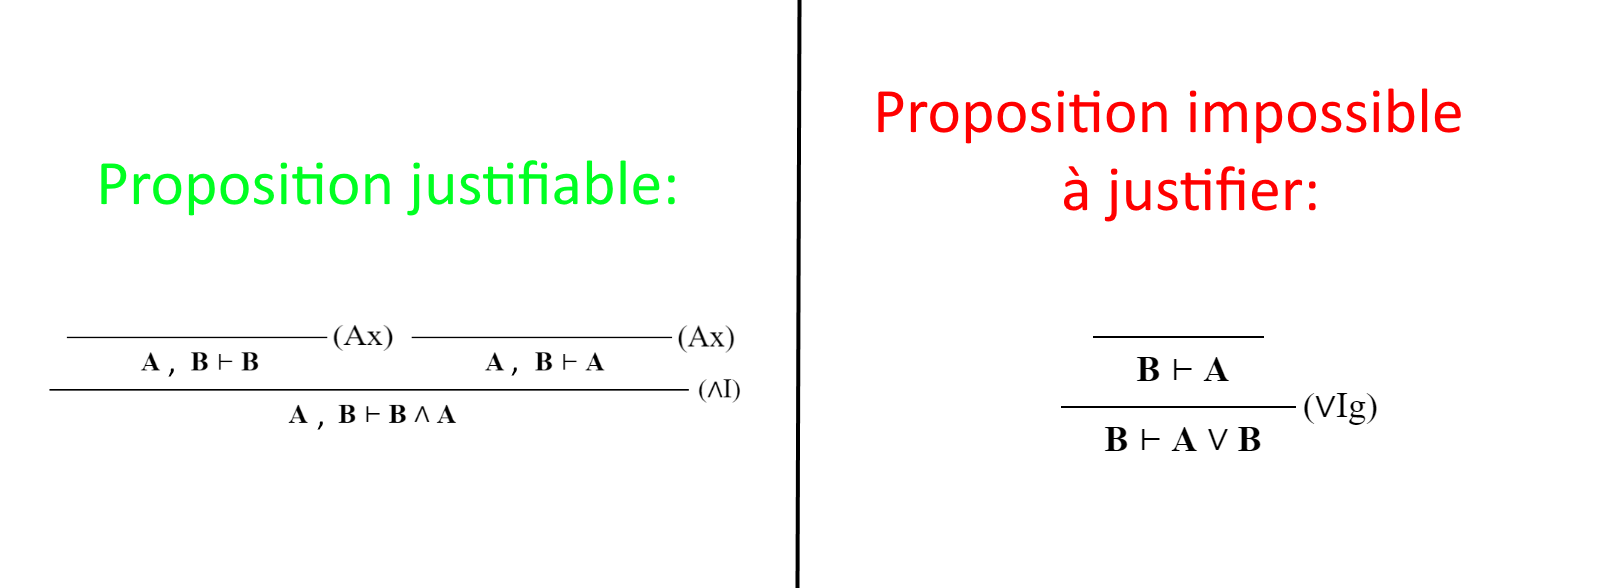
\includegraphics[scale=0.3]{schema1.png}
\end{center}
\caption{Certains blocs rendent la justification impossible}\label{im:blocs_et_ou}
\end{figure}
\FloatBarrier
Vous voyez bien ici qu'au départ, les deux proposition étaient justifiables.
L'introduction du \textit{et} nous a permis de finir la preuve.
Alors que l'introduction du \textit{ou} rend la proposition impossible à justifier.
L'introduction du \textit{ou} est donc à manier avec plus de précautions que l’introduction du \textit{et}.



\section{Rejoindre une classe}



Vous serez sûrement amenés à faire vos exercices dans une "classe", créée par vos professeurs. Pour cela, ouvrez le bandeau latéral gauche, et sélectionnez l'onglet "classe"
\begin{figure}[h!]
\begin{center}
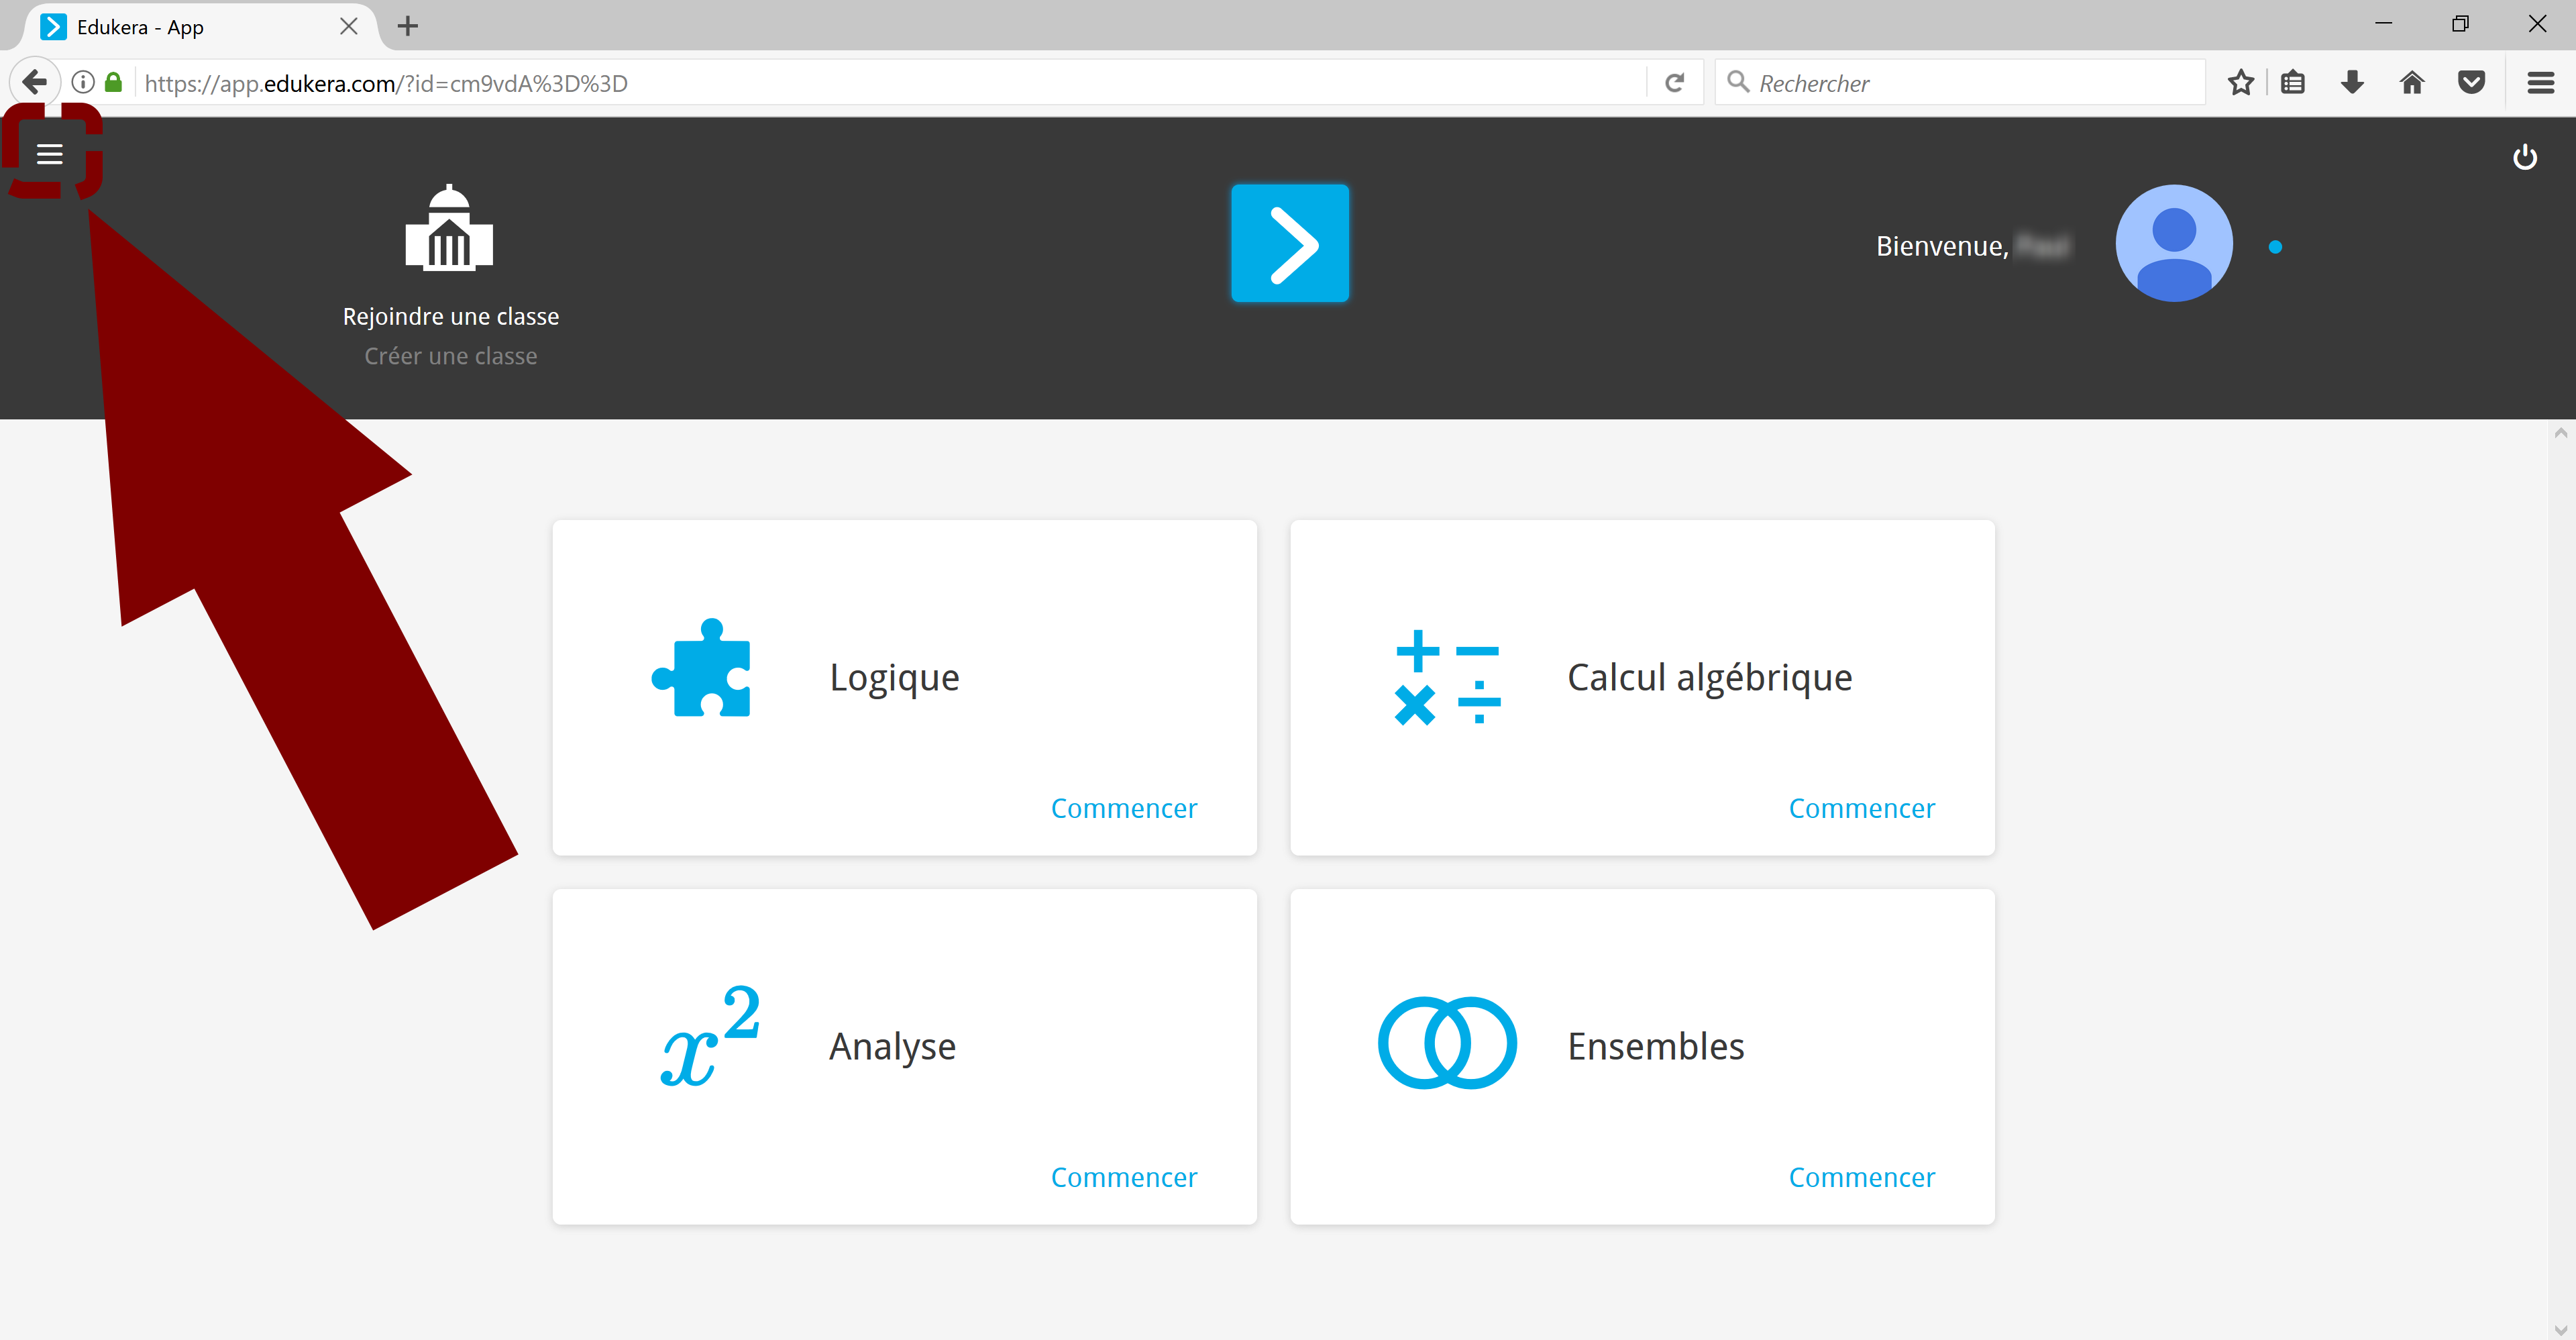
\includegraphics[scale=0.1]{img_app8.png}
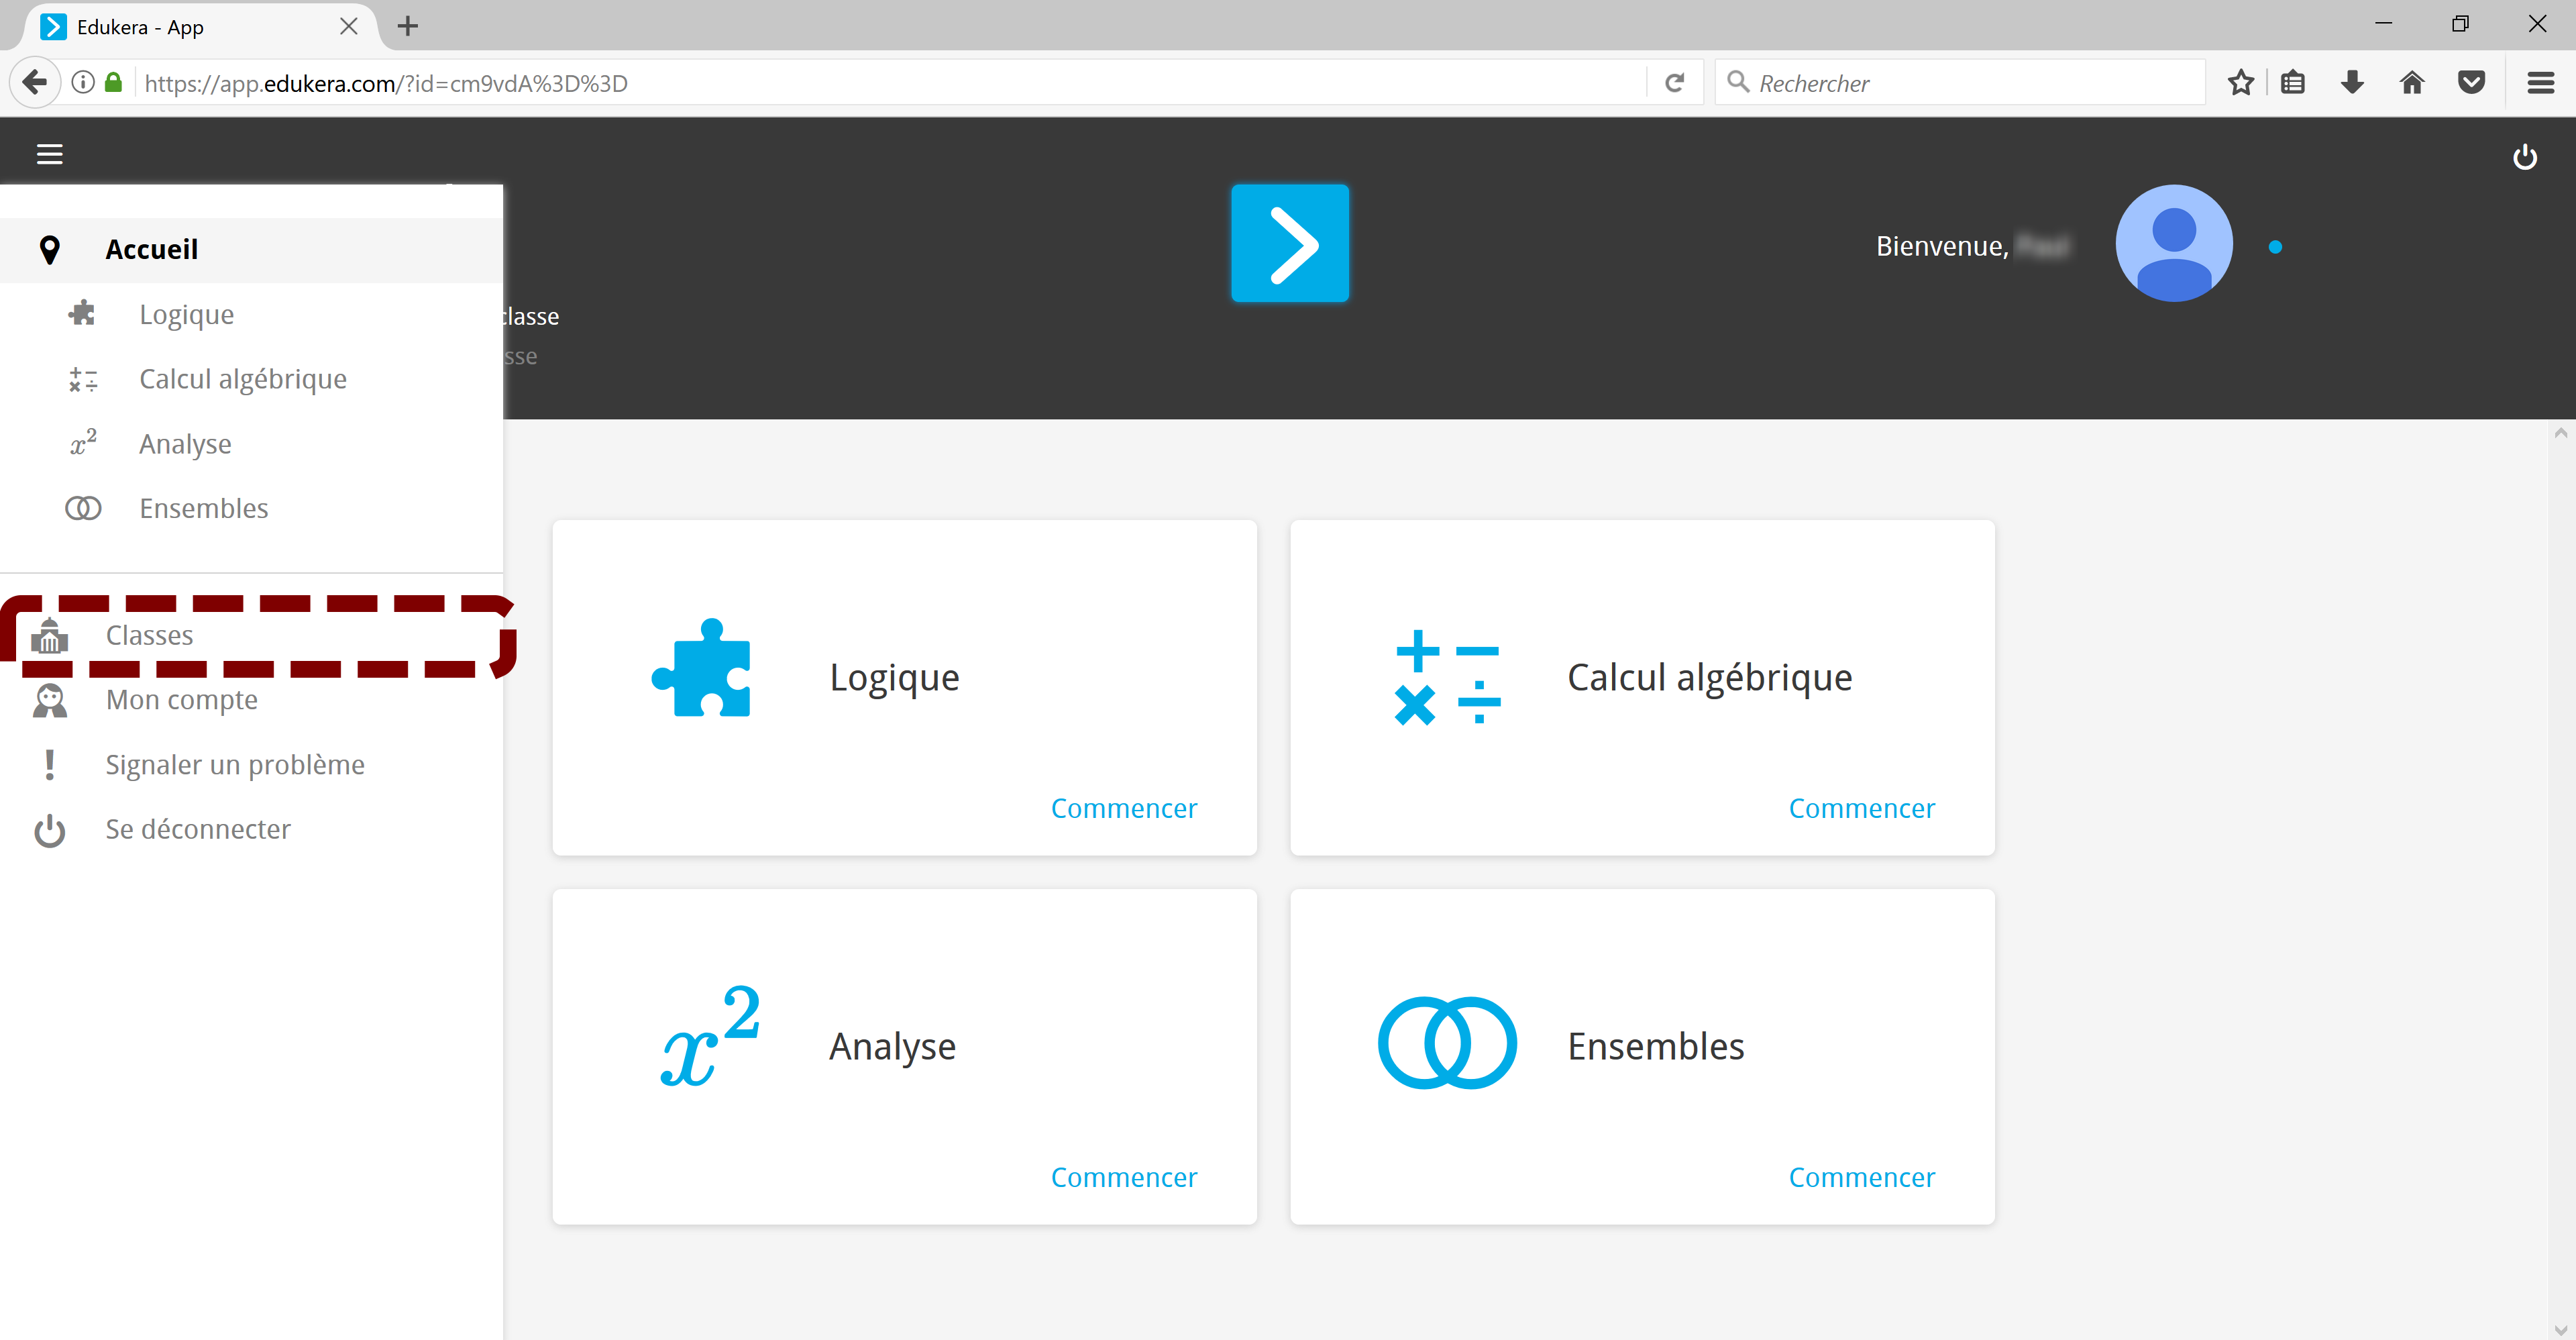
\includegraphics[scale=0.1]{img_app8bis.png}
\end{center}
\caption{Sélection d'une classe}\label{im:selec_classe}
\end{figure}
\FloatBarrier

Vous aurez ensuite un menu avec toutes vos classes, il ne vous restera plus qu'à cliquer dessus pour "entrer dans la classe".
Une classe se présent comme suit:



\subsection{Nuances entre votre exercices et les différents types de contrôles}



\begin{figure}[h!]
\begin{center}
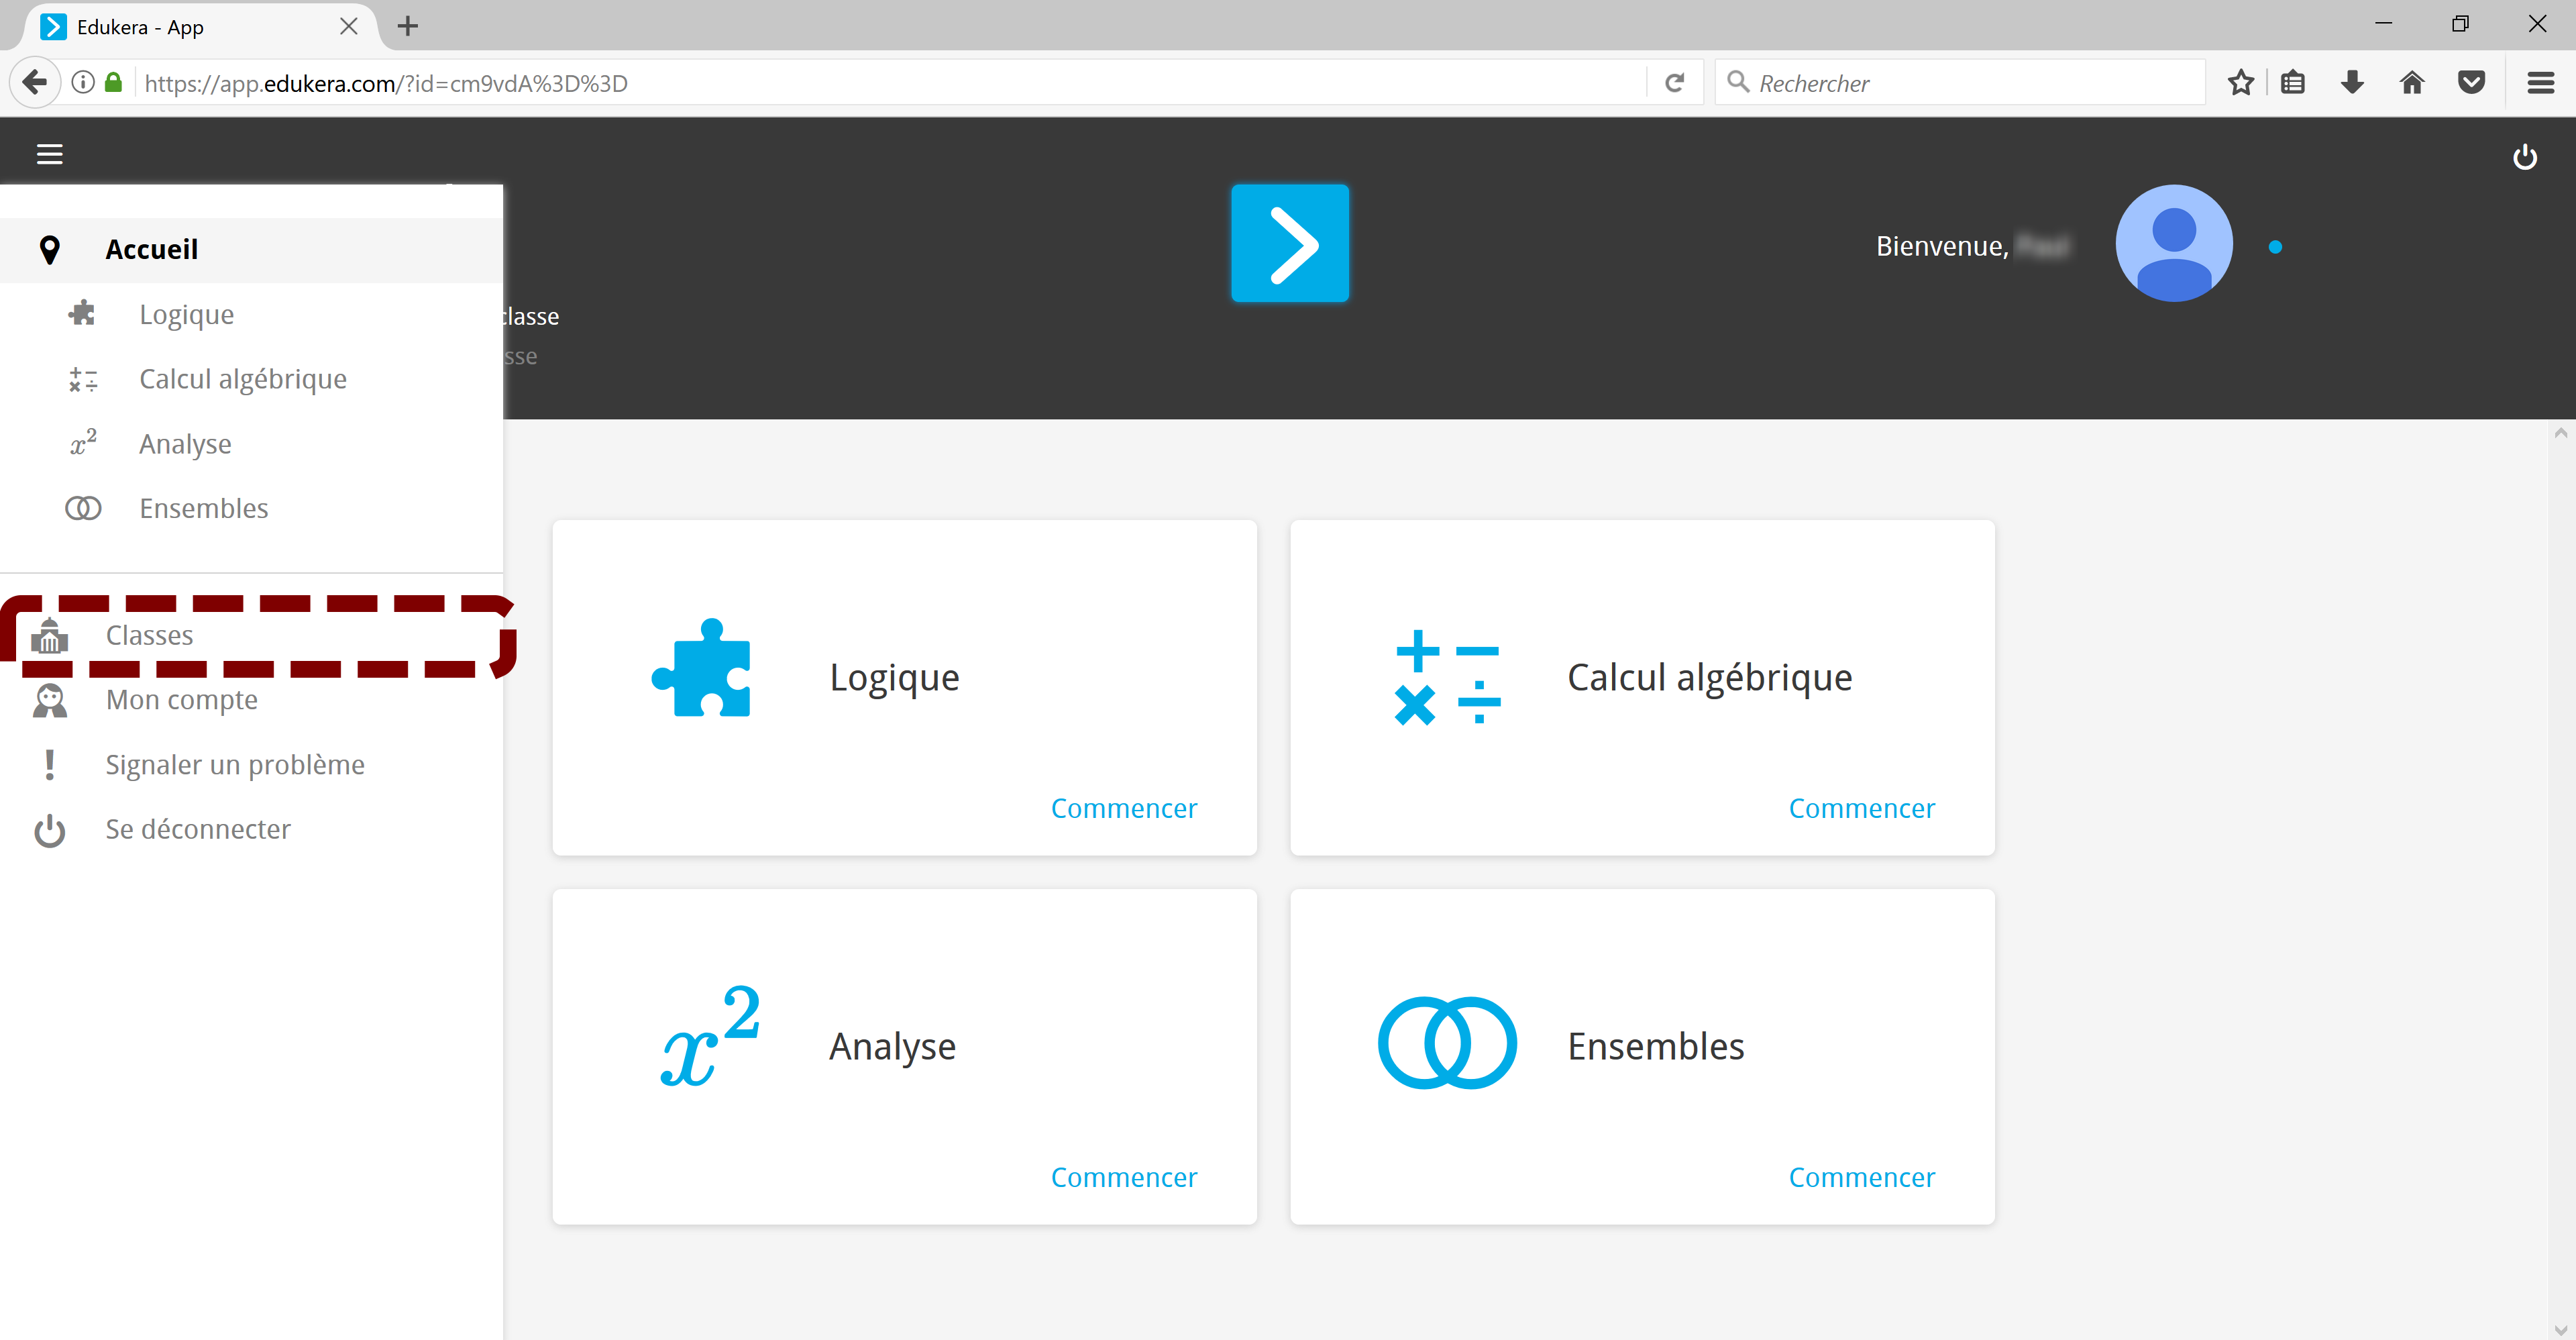
\includegraphics[scale=0.1]{img_app9.png}
\end{center}
\caption{Deux parties d'une classe}\label{im:parts_classe}
\end{figure}
\FloatBarrier

Vous remarquerez qu'il y a deux parties:
\begin{itemize}
\item \textbf{Exercices:} dans cette partie, il n'y a que les exercices sélectionnés par vos professeurs;
\item \textbf{Contrôles:} dans cette partie, il y a les contrôles et devoirs maisons (aussi sélectionnés par vos professeurs).
\end{itemize}
Dans la partie 'contrôles', vous remarquerez qu'ils sont de deux types:
\begin{itemize}
\item \textbf{les exercices notés:} les exercices que les étudiants doivent résoudre pendant leur temps libre; il y a la possibilité d'assigner une date de rendu qui sera prise en compte dans l'établissement de la note.
\item \textbf{les devoirs en temps limité:} Permet aux professeurs de faire un examen en salle machine; vos n'aurez pas accès aux exercices en dehors de la plage horaire définie.
\end{itemize}



\subsection{Nuances entre votre compte et la classe}


\todo[color=green!20,inline]{ \textbf{Attention!}  Si vous faites les exercices depuis
  l'accueil, ils seront marqués comme non faits dans la classe. Donc vos
  professeurs ne pourront pas voir votre travail!  Vous n'aurez pas d'autres
  choix que de les refaire, ce qui peut être frustrant.  D'autres part, depuis
  l'accueil, vous aurez accès à tous les exercices proposés par Edukera. Dans
  la classe, les exercices sont sélectionnés par le professeur, il y en a donc
  moins. Ne vous tropez pas si on vous dit "faites tous les exercices sur
  Edukera", il peut s'agir des exercices disponibles dans la classe
  uniquement.  }



\section{Pour aller plus loin}



Il est très fortement conseillé de maîtriser la partie connecteurs de la logique (l'interface n'est pas évidente à adopter...) pour comprendre les autres rubrique, cependant, il n'est pas nécessaire d'avoir fait tous les exercices.
Lorsque vous explorerez la partie quantificateurs, vous rencontrerez des règles qui nécessitent de sélectionner un élément.
Il suffit de cliquer sur une élément (a, b ...), et celui-ci sera sélectionné pour appliquer la règle:
\begin{figure}[h!]
\begin{center}
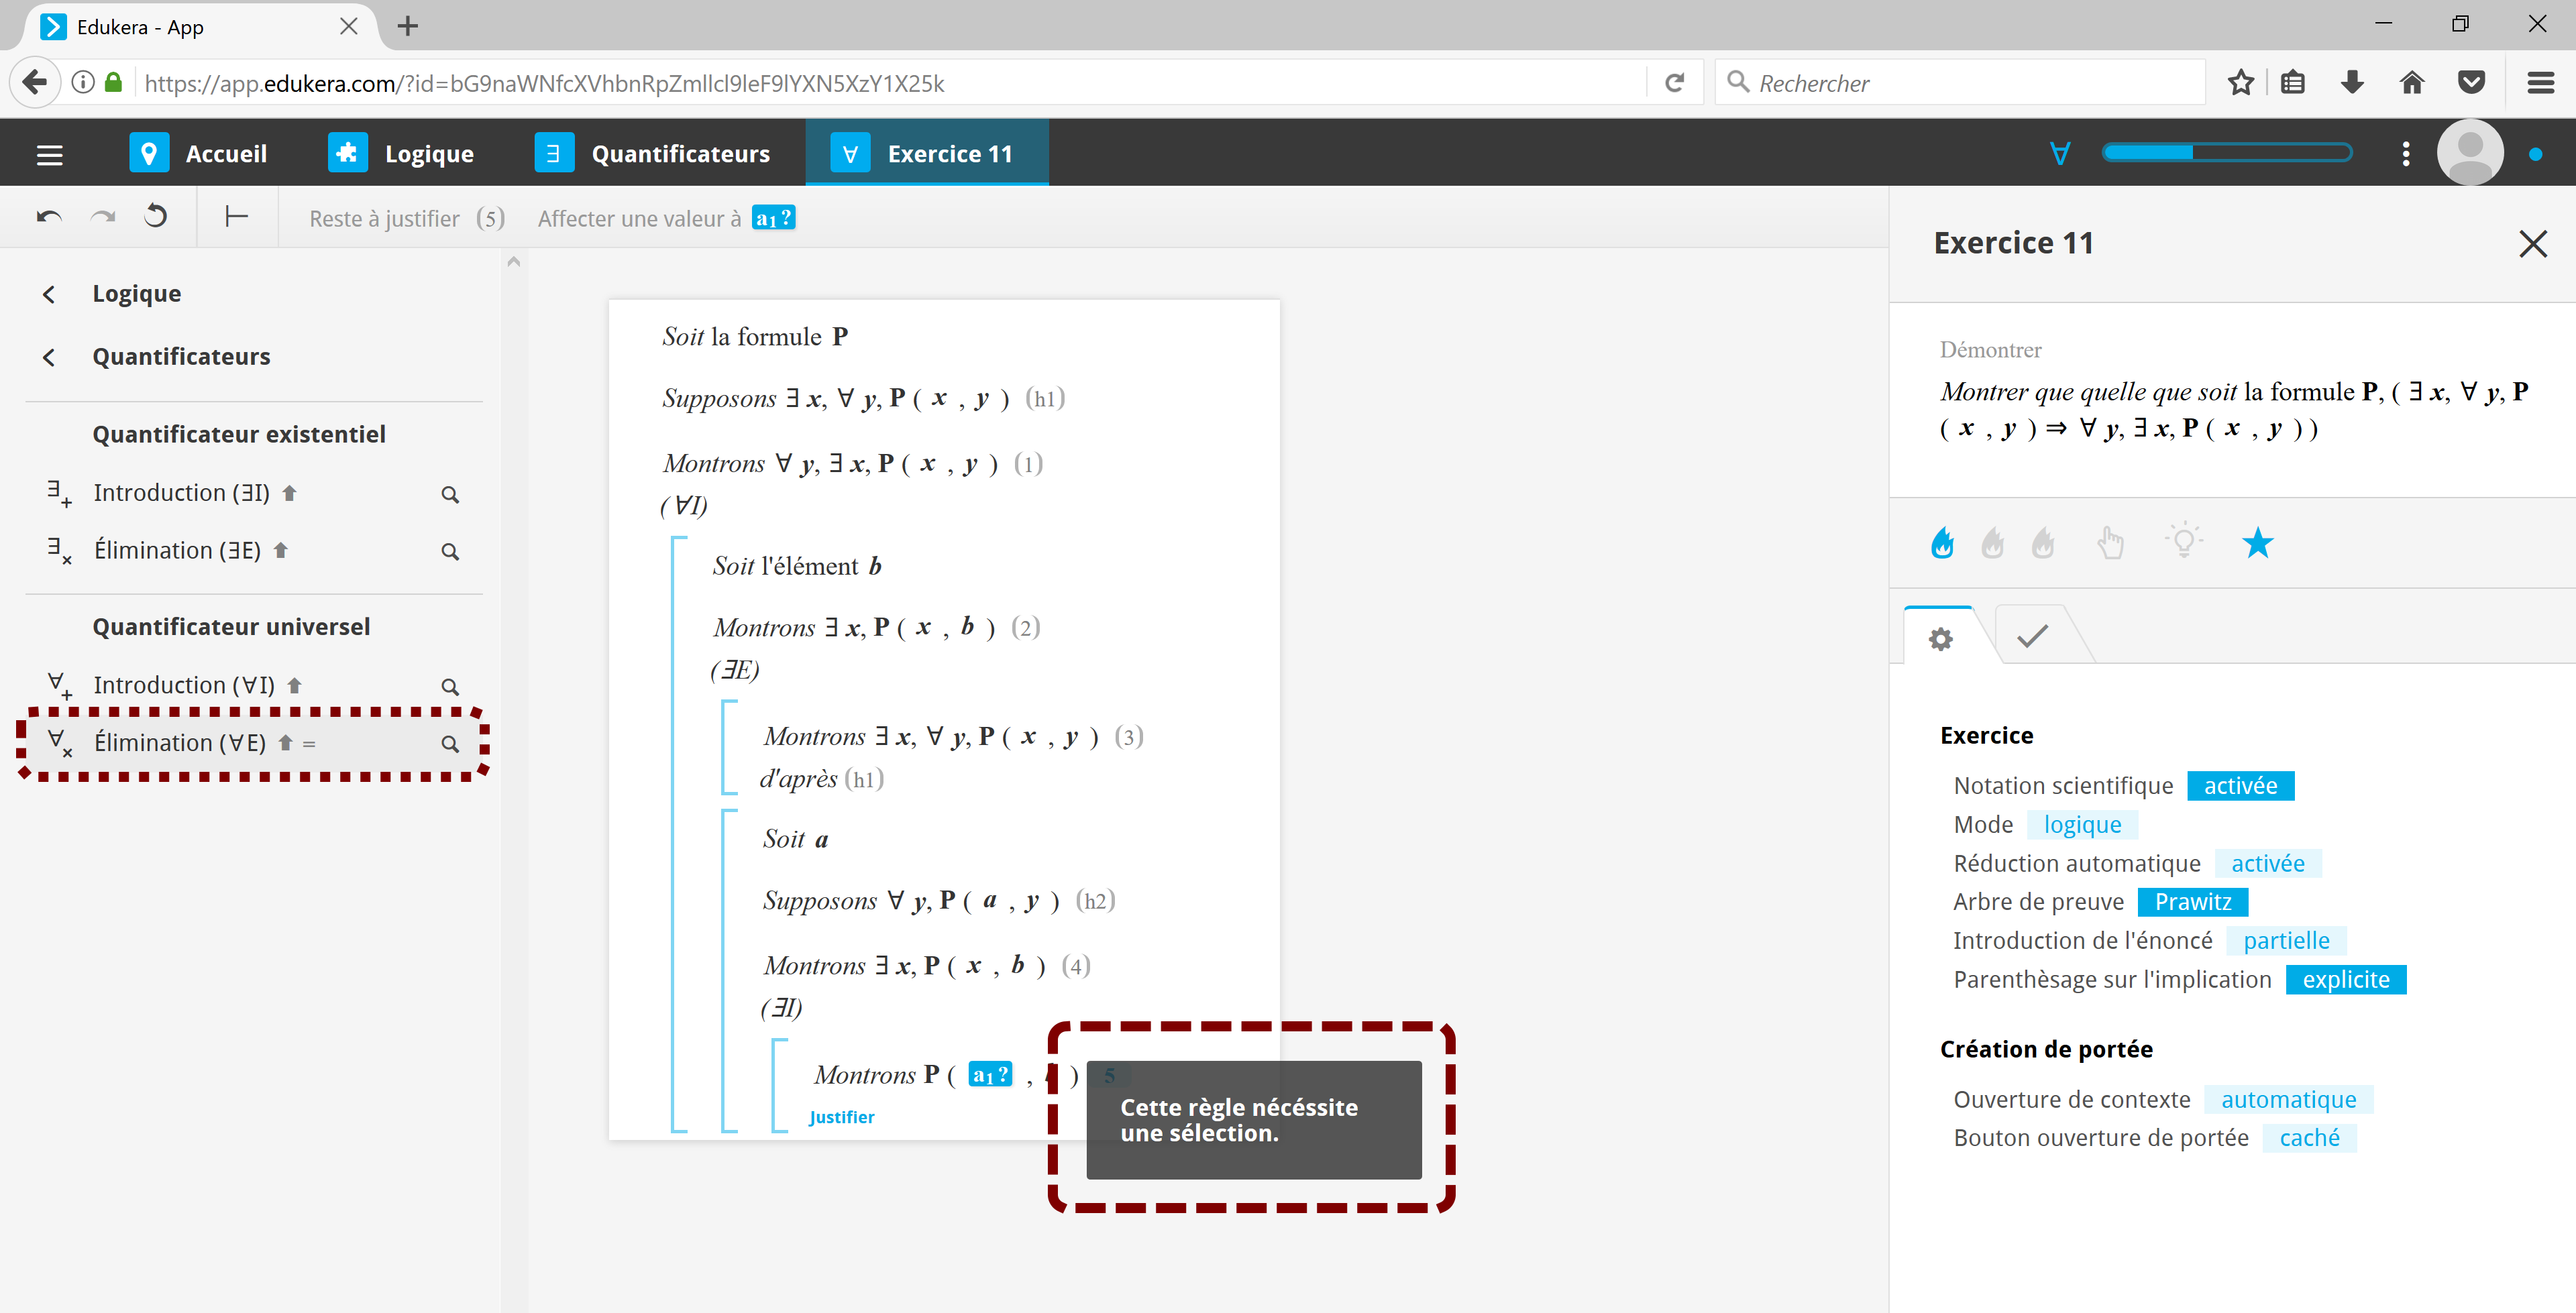
\includegraphics[scale=0.1]{img_app10.png}
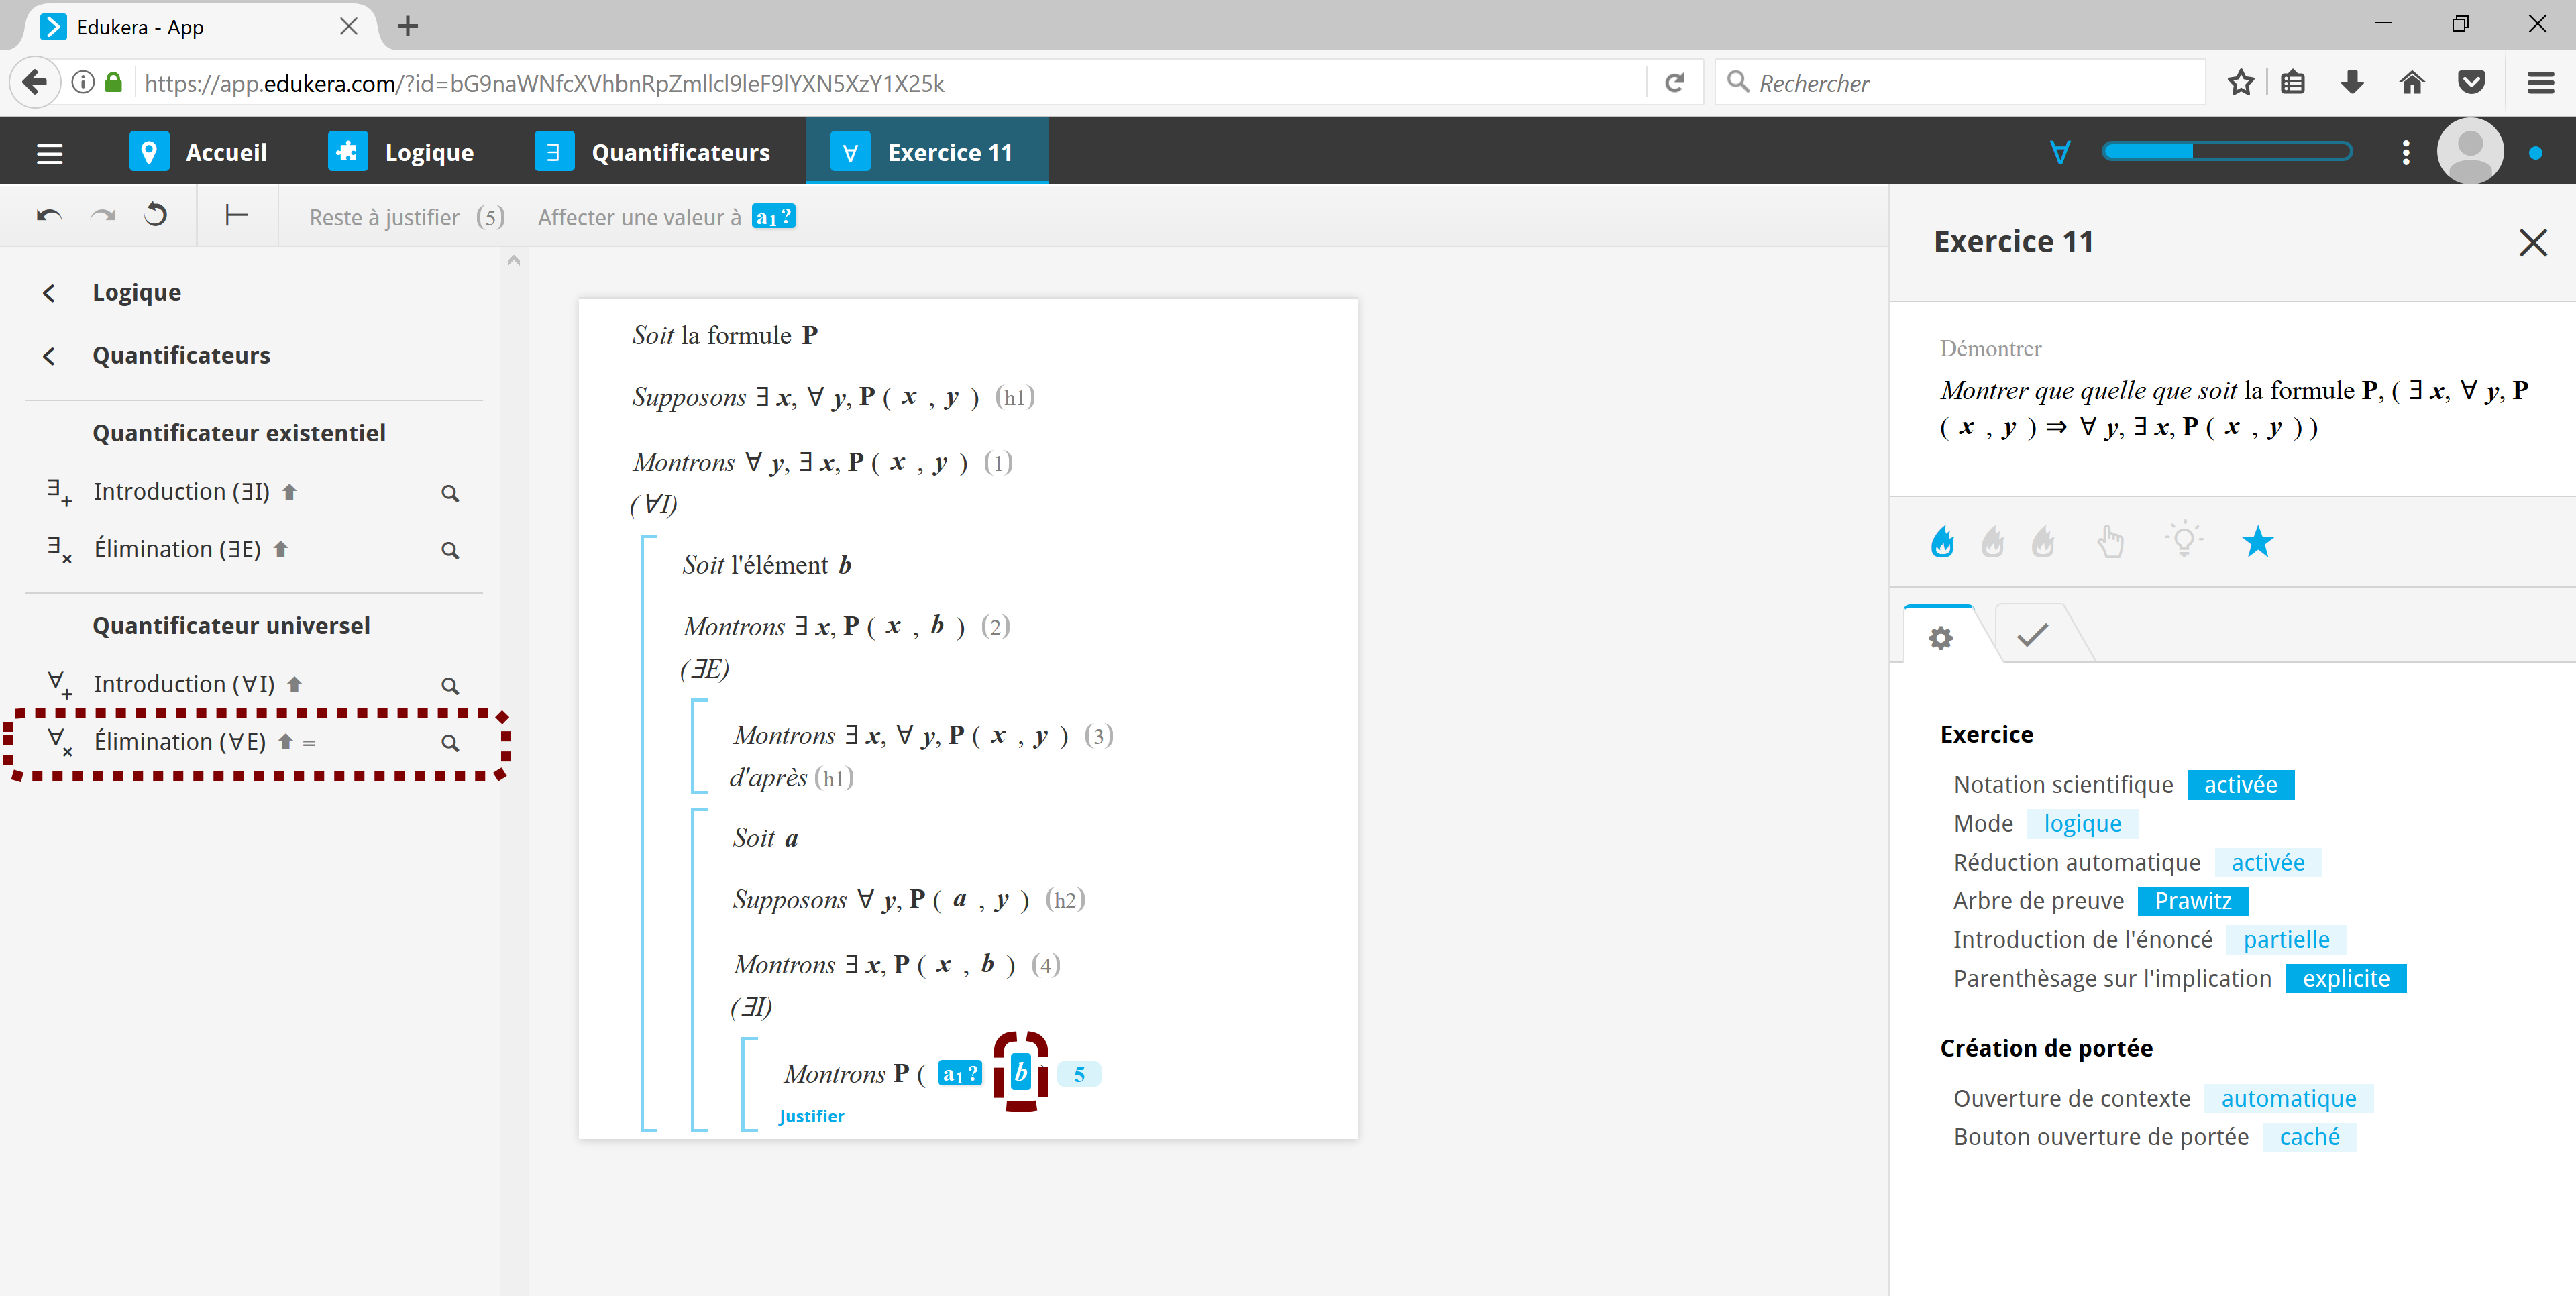
\includegraphics[scale=0.1]{img_app11.png}
\end{center}
\caption{Sélection d'un élément}\label{im:selec_elem}
\end{figure}
\FloatBarrier



\todo[color=red!20,inline]{ \textbf{TIP: } Les exercices que vos prof ont sélectionné pour les contrôles sont sûrement pas désactivés dans les exercices de la classe, mais tous les exercices sont disponibles depuis l'accueil de votre compte. En recoupant les exercices présents dans la classe et depuis l'accueil du compte, il est peut-être possible de connaître à l'avance des exercices du contrôle, et de les réviser auparavant... ;) }



\end{document}